\chapter{ПРОЕКТИРОВАНИЕ СИСТЕМЫ УПРАВЛЕНИЯ ДВИЖЕНИЕМ БЕСПИЛОТНОГО АВТОМОБИЛЯ}
В данной главе рассматривается этап проектирования структуры и алгоритмов системы управления движением беспилотного
автомобиля. Проектирование системы основано на анализе рассмотренных архитектурных решений и алгоритмов.

\section{Формулирование требований к разрабатываемой системе}


Система управления беспилотным автомобилем должна выполнять большое количество функций, необходимых для эффективного
и безопасного движения в сложных условиях, среди которых
\begin{itemize}
    \item распознавание других участников дорожного движения (автомобилей, пешеходов,
          велосипедистов и т.п.);
    \item отслеживать других участников дорожного движения в течении некоторого времени для определения характеристик
          их движения и уменьшения ошибок распознавания;
    \item определять положение, скорость, ускорение и предсказывать будущие действия других участников дорожного
          движения;
    \item распознавать дорожные знаки, светофоры;
    \item распознавать дорожную разметку;
    \item на основании всей собранной информации осуществлять планирование безопасного и эффективного движения;
    \item выполнять запланированное движение и реагировать на изменения в дорожной ситуации.
\end{itemize}

Исходя из требуемой функциональности, а так же критериев безопасности, система управления беспилотным автомобилем
обладает высочайшей сложностью. Разработку такой системы невозможно осуществить в полной мере сразу, по "водопадной"
модели. Различные компоненты системы должны разрабатываться и улучшаться независимо, чтобы наращивать функциональность
и увеличивать безопасность и эффективность системы управления.

Поэтому главным требованием к системе управления беспилотным автомобилем является высокая модульность, что позволит
разрабатывать и тестировать отдельные системы и подсистемы независимо.

Другим требованием, также приводящим к необходимости модульной системы, является необходимость иметь возможность
тестирования компонентов системы управления беспилотным автомобилем на небольших моделях и с использованием различных
симуляторов и иных средств моделирования, что позволит быстрее приступить
к разработке системы, не завися от реализации системы управления органами управления реального автомобиля.

В связи с очень большим объемом работ, требуемом для разработки полной системы управления беспилотного автомобиля, в
рамках данной работы будет осуществляться разработка небольшой части требуемой функциональности:
\begin{itemize}
    \item осуществление движения по заданной траектории с обратной связью;
    \item осуществление локального планирования, чтобы формировать оптимальные или близкие к ним траектории движения,
          позволяющие достичь поставленной локальной цели;
    \item прототип системы распознавание препятствий, способный распознавать простейшие статические препятствия,
          для того, чтобы экспериментально проверить предыдущие две возможности;
    \item управление исполнительными органами мобильной платформы для выполнения запланированных движений.
\end{itemize}

\section{Проектирование общей архитектуры системы управления движением}

Разрабатываемую в рамках данной работы систему управления можно разделить на несколько частей: драйвер автомобиля,
система распознавания препятствий, система планирования локальной траектории и система следования по траектории.

Для отработки и тестирования системы управления необходимо построить небольшую мобильную платформу, которая будет
использоваться для проведения экспериментов. Мобильная платформа должна быть оснащена датчиками, используемыми для
распознавания препятствий и определения собственного положения в локальной системе координат, необходимого для
реализации движения по траектории с обратной связью. Платформа должна быть оснащена встраиваемым компьютером достаточной
производительности. Помимо этого, разумеется, необходимо осуществлять управление приводами платформы.

Для осуществления управления беспилотным автомобилем необходим ряд сенсоров, обеспечивающих систему управления
необходимой информацией об окружающей обстановке. Беспилотные автомобили, разрабатываемые крупными компаниями
оснащены множество сенсоров, описанных в первой главе. Основными типами сенсоров являются камеры, LiDAR, радары,
GPS и другие.

Система компьютерного зрения является одним из самых сложных и критичных компонентов системы управления беспилотного
автомобиля, от надежности и работы которой зависит безопасность автомобиля и других участников дорожного движения.
Разработка системы компьютерного зрения, которая в полной мере удовлетворяет этим требованиям ~--- крайне сложная и
ресурсоемкая задача, над решением которой в течении многих лет работают ведущие компании-разработчики беспилотных
автомобилей и, тем не менее, эта задача далека от полного решения.

Все современные, start-of-the-art, системы компьютерного зрения используют глубокие нейронные сети для решения таких
задач, как детектирование объектов, детектирование дороги (области доступной для движения), детектирования дорожной
разметки, детектирования светофоров и дорожных знаков, предсказания намерений других участников движения. В этих задачах
глубокие нейронные сети давно являются стандартом де-факто и существенно превосходят по точности распознавания любые
классические алгоритмы. Тем не менее, использование технологий машинного обучения, в частности, глубоких нейронных
сетей, приводит к дополнительным трудностям. Помимо разработки архитектуры нейронной сети, поиска ее параметров, крайне
важную роль играют данные, используемые для обучения нейронной сети. Именно данные играют критическую роль в том, как
система компьютерного зрения будет выполнять свою работу, особенно в сложных условиях и редких ситуациях. Добиться
правильного поведения нейросетевого алгоритма в тех ситуациях, когда он ошибается, можно только с помощью предоставления
дополнительных обучающих данных, покрывающих этот случай. Крупные компании, обладающие доступом к огромным массивом
данных имеют значительное преимущество в этой области. Так, например, компания Tesla, располагает парком из сотен
тысяч автомобилей, которые предоставляют телеметрию, позволяя определять ситуации, в которых работа автопилота была
некорректна, собирать похожие ситуации, записанные автомобилями по всему миру, и оперативно дообучать используемые
нейронные сети.

В связи с высокой сложностью разработки системы компьютерного зрения, в данной работе не рассматривается разработка
полноценной системы компьютерного зрения. Тем не менее, с целью отладки алгоритмов планирования движения и движения
по траектории, необходимо разработать простую систему компьютерного зрения, которая бы решала следующи задачи:
\begin{itemize}
      \item определение положения и ориентации модели автомобиля с точностью, достаточной для работы регулятора с
            обратной связью ддя точного движения по траектории;
      \item определение статических препятствий, с целью проверки системы объезда препятствий.
\end{itemize}

Для реализации первой задачи было решено применять алгоритм одновременной картографии и навигации (SLAM) на основе
стереозрения. SLAM-алгоритмы не позволяют получать глобальное положение автомобиля и подвержены накоплению ошибок при
передвижении на большие расстояния, но для проверки задачи локального планирования движения они хорошо подходят, потому
что обеспечивают высокую точность позиционирования и частоту обновления данных.

Для определения препятствий было решено использовать шестнадцатилучевой LiDAR Velodyne VLP-16, который был приобретен
для проекта беспилотного автомобиля и предполагался для установки на полноразмерный автомобиль. LiDAR позволяет получить
трехмерное облако точек, представляющее окружающую обстановку, обладающее сравнительно большой детализацией, обнаруживая
препятствия на расстояниях до ста метров. Использование LiDAR для малой мобильной платформы кажется избыточным, но
качественное облако точек, которое он предоставляет, существенно облегчает задачу обнаружения препятствий.

Диаграмма компонентов системы управления беспилотным автомобилем представлена на рисунке
\ref{img:system_component_diagram}. Все компоненты можно разделить на следующие группы:
\begin{itemize}
      \item драйверы сенсоров, осуществляющие работу с сенсорами, такими как LiDAR и камеры, и предоставляющие
            API для удобного получения данных другими компонентам системы управления;
      \item основные компоненты системы управления, осуществляющие основную работу по восприятию окружающей
            обстановки, планированию и управлению движением;
      \item драйверы исполнительных устройств автомобиля, позволяющие исполнять сформированные последовательности
            команд непосредственно аппаратным оборудованием автомобиля.
\end{itemize}

\begin{figure}[h]
      \centering
      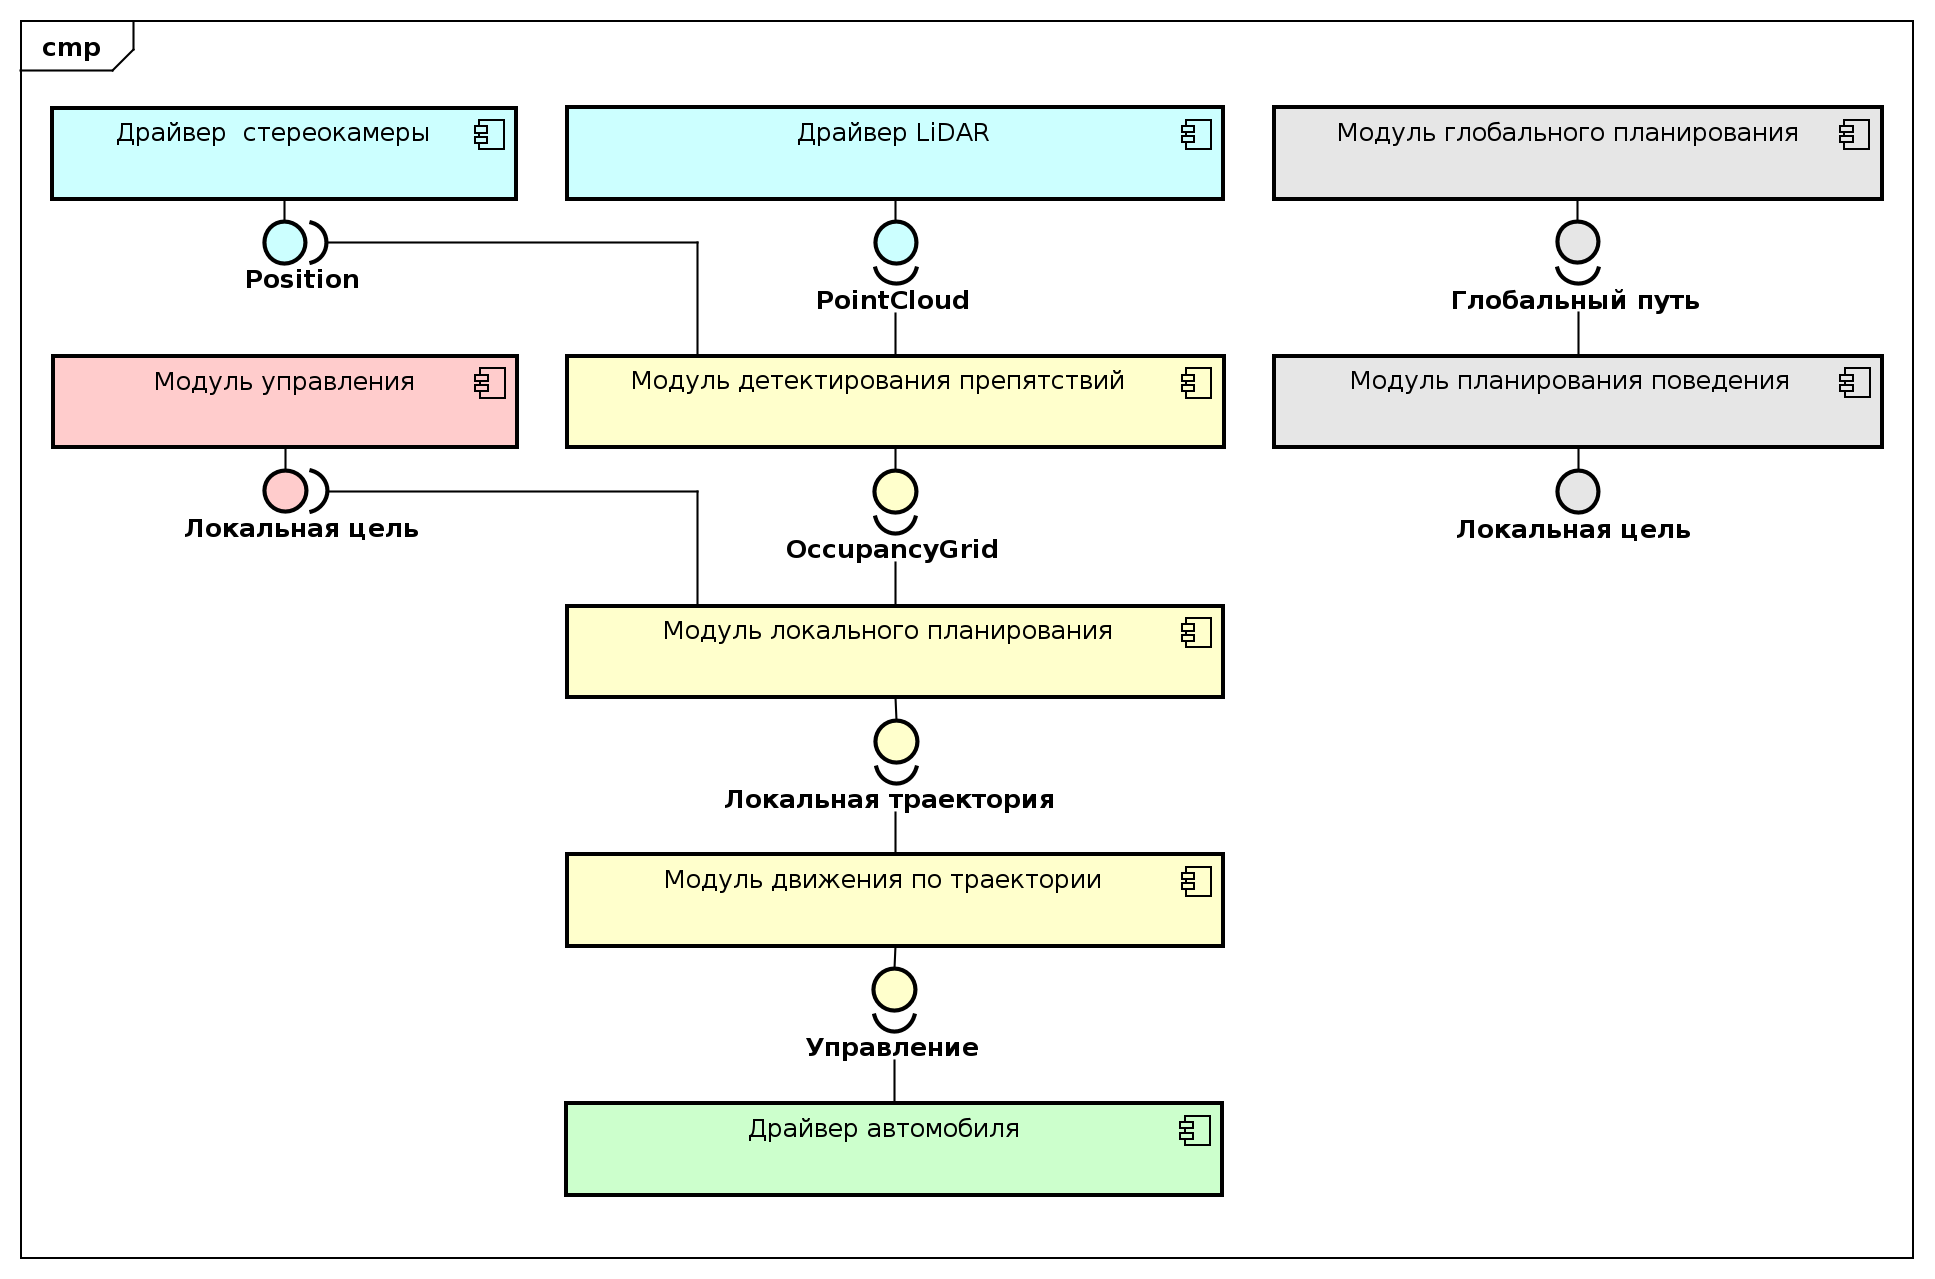
\includegraphics[width=\linewidth]{images/system_component_diagram}
      \caption{Диаграмма компонентов системы управления беспилотным автомобилем}
      \label{img:system_component_diagram}
  \end{figure}

Драйвер стереокамеры реализует работу со стереокамерой и алгоритм SLAM. Этот модуль предоставляет данные о текущем
положении и ориентации автомобиля в локальной системе координат. Драйвер LiDAR предоставляет облако точек, полученное
с LiDAR. Модуль детектирования препятствий осуществляет базовое детектирование препятствий в полученном облаке точек
и представляет информацию о них в виде т.н. Occupancy Grid. Occupancy Grid - это распространенный способ представления
информации о препятствиях в виде регулярной двухмерной сетки, каждая ячейка которой может быть в одном из трех
состояний: свободно, препятствие или неизвестно. Система управления беспилотным автомобилем в общем виде имеет модули
глобального планирования и планирования поведения, которые отвечают за построение глобальной траектории по дорожной
сети и принятие решений в соответствии с окружающей обстановкой и правилами дорожного движения, как было рассмотрено
в первой главе \ref{img:general_arch}. В рамках данной работы эти модули не рассматриваются и заменяются пользовательским
интерфейсом оператора, с помощью которого можно вручную указать локальную цель, вместо того, чтобы она задавалась
планировщиком поведения. На основании локальной цели, текущего положения автомобиля, полученного от модуля SLAM, и
инофрмации о препятствиях, полученных от модуля распознавания препятствий, модуль планирования локальной траектории
осуществляет планирование локальной траектории, которая позволит автомобилю достичь (если это возможно), поставленной
локальной цели. Сформированный локальным планировщиком путь поступает на вход регулятора с обратной связью, который
осуществляет управление исполнительными механизмами автомобиля, чтобы удерживать автомобиль на заданной траектории,
получая в качестве обратной связи текущее положение, ориентацию и скорость от модуля SLAM.

\section{Проектирование подсистемы планирования локальной траектории}
Основной системой, разрабатываемой в рамках этой работы, является система планирования локальной траектории. Эта система
получает очередную цель от системы планирования поведения и осуществляет формирование оптимальной или близкой к нему
достижимой траектории для достижения этой цели. Достижимость подразумевает, что полученная траектория не приведет к
столкновению с известными препятствиями, с учетом габаритов препятствий и автомобиля, а также выполнима для автомобиля
с точки зрения его кинематики и динамики движения.

Существует большое количество различных алгоритмов планирования движения, ряд из которых был рассмотрен и проанализирован
в первой главе. Наиболее распространенными группами методов являются методы поиска на графах, включая различные
модификации, направленные на планирование достижимых для автомобиля путей, такие как методы решетки состояний
(state lattice), и методы интерполяции кривых. Первые являются более универсальными, и применяются в том числе для
планирования в неструктурированном окружении. Вторые больше ориентированы на планирование движения по дорогам, что
накладывает ряд ограничений, упрощающих задачу планирования движения.

В данной рамках данной работы реализуется метод планирования движения по дороге. \hl{Ну и почему?}

\subsection{Использование алгоритма A*}
Первоначальный вариант алгоритма планирования локальных траекторий основывался на алгоритме A*. Причиной
выбора этого алгоритма послужило то, что это простой  и распространенный алгоритм для нахождения пути
на графах, в частности, он широко применяется для работы с Occupancy Grid.

Для работы алгоритм требует опорную траекторию, которая используется в качестве начального приближения, а затем
модифицируется, чтобы избежать столкновения с препятствиями.

Таким образом, планировщик поведения или, в случае данной работы, графический интерфейс оператора, должны предоставлять
опорную траекторию, помимо требуемого целевого состояния. Это требует дополнительной работы от планировшика поведения
и не позволяет сделать интерфейс локального планировщика полностью абстрактным, не зависящим от его реализации, потому
что не всем возможным реализациям требуется опорная траектория (например, алгоритмам на основе RRT она не требуется).
Тем не менее, это не является значительным препятствием. Опорная траектория при движении по непрерывному сегменту дороги
может быть реализована как центральная линия текущей полосы, по которой движется автомобиль. Это может быть определено
с помощью системы компьютерного зрения. Для более сложных ситуаций, например, перекрестков, подобная траектория может
быть реализована в виде сплайна, соединяющего соответствующие полосы двух пересекающихся дорог.

Алгоритм работает следующим образом. Рассматривается ближайший участок опорной траектории определенной длины, и если
на этому участке опорная траекторий пересекается с препятствием, то запускается алгоритм обхода препятствия, в противном
случае продолжается движение по опорной траектории. Для обхода препятствия ищется точка на опорной траектории,
где заканчивается препятствие (в случае, если это нельзя определить, например, препятствие закрывает обзор системе
компьютерного зрения, берется некий допуск от последних видимых клеток препятствий на Occupancy Grid). После этого
запускается алгоритм A* для нахождения пути от текущего положения автомобиля до точки выхода опорной траектории из
зоны препятствия. Алгоритм запускается с определенной периодичностью и перестраивает траекторию, таким образом, по
мере движения автомобиля системе компьютерного зрения становятся обозримы новые участки препятствия и траектория
перестраивается.

Этот алгоритм обладает серьезными недостатками:
\begin{itemize}
      \item не учитывает кинематику и динамику автомобиля;
      \item не планирует скорость движения.
\end{itemize}

Алгоритм был реализован и испытан на мобильной платформе. По результатам испытаний были выявлены дополнительные
недостатки алгоритма. В связи с неидеальностью системы компьютерного зрения, при обновлении периодическом Occupancy Grid
происходит небольшое "мерцание", т.е. те или иные пограничные ячейки карты могут менять свое состояние. Это приводит
к тому, что алгоритм резко перестраивает траекторию движения. Особенно это было заметно, когда модель приближалась
к симметричному препятствию. В таком случае, алгоритм мог прокладывать обходную траекторию то по левую сторону от
препятствия, то по правую сторону от препятствия. Это приводило к тому, что модель не могла корректно осуществить
маневр и врезалась в препятствие.

По результатам испытаний было выявлено, что рассмотренный алгоритм не подходит для локального планирования траекторий
движения беспилотного автомобиля.

\subsection{Метод интерполяции кривых}
Исходя из результатов испытания алгоритма на основе A*, было принято решение разработать другой алгоритм. За основу для
проектирования системы планирования локальной траектории был выбран метод, предложенный командой "Junior" Darpa
Urban Challenge \cite{darpa_junior}, который был кратко рассмотрен в главе 1. Преимуществами этого подхода
являются:
\begin{itemize}
      \item лучший учет кинематических и динамических ограничений автомобиля за счет планирования траектории в
            виде гладких кривых;
      \item применение полиномов пятого порядка позволит планировать гладкие траектории с гладкой первой производной
            (скоростью), благодаря чему не будет осуществляться резкая перестройка траектории;
      \item алгоритм позволяет находить оптимальные или близкие к оптимальным траектории, в отличие от, например,
            алгоритмов на основе RRT;
      \item алгоритм обладает меньшей вычислительной сложностью, чем алгоритмы на основе RRT.
\end{itemize}

Основным недостатком данного алгоритма является то, что в нем нет настоящего учета динамической модели автомобиля.
Для учета динамических ограничений применяются косвенные признаки, такие как максимальные продольные скорость и ускорение,
максимальное боковое ускорение, минимальный радиус кривизны, которые могут быть получены в результате анализа динамической
модели автомобиля. Для обеспечения соблюдения этих условий в широком диапазоне различных условий приходится устанавливать
эти ограничения с запасом. Это приводит к тому, что динамические возможности автомобиля используются не полностью.
Нарушение динамических ограничений также не исключено, например, при смене условий (например, мокрая дорога), что
может снизить безопасность автомобиля. Тем не менее, при выборе достаточно жестких ограничений, можно обеспечить
высокую надежность этого алгоритма. Алгоритм хорошо зарекомендовал в соревновании DARPA Urban Challenge \cite{darpa_junior}.

Для работы методы необходимы следующие входные данные:
\begin{itemize}
      \item опорная (рефернсная) траектория;
      \item локальная цель, описывающая требуемое положение и скорость автомобиля, эта точка должна
            лежать на опорной траектории;
      \item текущее состояние автомобиля (положение, скорость, ускорение);
      \item карта препятствий в формате Occupancy Grid.
\end{itemize}

Этот алгоритм, как и предыдущий, требует получения от планировщика поведения опорной траектории, помимо целевого
состояния.

Планирование траектории осуществляется независимо для продольного движения вдоль опорной траектории и поперечного
движения. Планирование осуществляется в подвижной системе координат, движущейся по опорной траектории вместе с
автомобилем, как показано на рисунке \ref{img:frenet_frame}.

\begin{figure}[h]
      \centering
      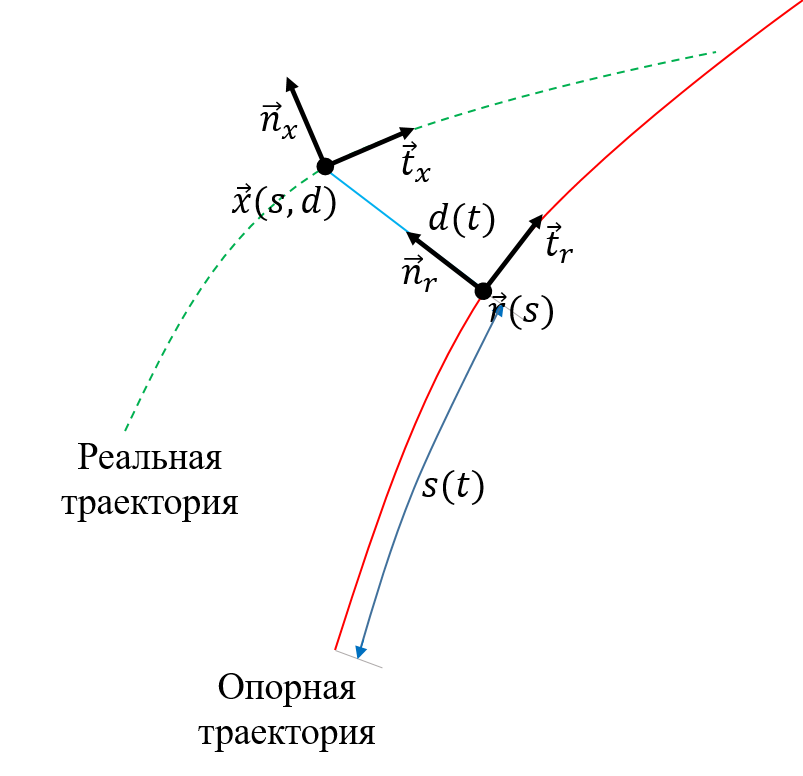
\includegraphics[]{images/frenet_frame}
      \caption{Диаграмма компонентов системы управления беспилотным автомобилем}
      \label{img:frenet_frame}
\end{figure}

Опорная траектория (изображена на рисунке красной линией) представлена натурально параметризованная кривая, где $s(t)$
~--- покрытая длина дуги в момент времени $t$. Положение автомобиля в глобальной системе координат обозначено
радиус-вектором $\vec{x}$. Этому положению автомобиля соответствует подвижная система координат $\vec{r}(s)$,
представляющая собой ортонормированный репер Френе, где $\vec{t}_r$ и $\vec{n}_r$ ~--- касательный и нормальный вектора
к опорной траектории соответственно. Таким образом, положение автомобиля в глобальной декартовой системе кординат
$(x, y)$ может быть представлено в подвижной системе координат как $(s, d)$, где $d$ - расстояние между автомобилем и
опорной траекторией.

Продольная и поперечная траектории движения ищутся в форме полиномов пятого порядка, соединяющие начальное состояние
(текущее состояние автомобиля, полученное от сенсоров) и целевое состояние (полученное от планировщика поведения или
графического интерфейса оператора). Первые и вторые производные этих
полиномов представляют собой зависимость скорости и ускорения автомобиля от времени, которые затем подаются в регулятор
с обратной связью наряду с пространственной траекторией движения, т.е. этот метод позволяет планировать не только
траекторию перемещения автомобиля, но и профиль скорости.

Задача состоит в том чтобы найти коэффициенты полинома, которые минимизируют некую функцию стоимости, используемую для
оценки траекторий. За основу для функции стоимости взят интеграл производной ускорения по времени $\dddot{s}$,
называемая рывок (jerk). Это является распространенным выбором функции стоимости во многих алгоритмов планирования
движения автомобилей. Ниже представлены интегралы для продольного и поперечного движения соответственно:
\begin{equation}
      \label{eq:lon_jerk_integral}
      J_s = \int_{t_0}^{t_1}{\dddot{s}(t)^2dt}
\end{equation}
\begin{equation}
      \label{eq:lat_jerk_integral}
      J_d = \int_{t_0}^{t_1}{\dddot{d}(t)^2dt}
\end{equation}

\noindent\begin{tabularx}{\linewidth}{lllX}
      где & $s(t), d(t)$ &~---& функция продольной и поперечной траекторий соответственно, \\
          & $t_0, t_1$   &~---& начальное и конечное время маневра соответственно. \\
\end{tabularx}

Такой выбор функционала стоимости обоснован следующим:
\begin{itemize}
      \item минимизация количества и резкости маневров, совершаемых автомобилем (резкая траектория
            с большим количество маневров может быть получена в результате других алгоритмов
            планирования, таких как RRT), что повышает безопасность и экономичность движения;
      \item обеспечение комфорта пассажиров
\end{itemize}

В соответствии \cite{darpa_junior_frenet_origin} оптимальное решение, минимизирующее рывок, может быть найдено в форме
полиномов пятого порядка:
\begin{eqnarray}
      \label{eq:quntic_and_d}
      s(t)        =& a_0t^5   + a_1t^4 + a_2t^3 + a_3t^2 + a_4t + a_5 \\
      \dot{s}(t)  =& 5a_0t^4  + 4a_1t^3 + 3a_2t^2 + 2a_3t + a_4 \\
      \ddot{s}(t) =& 20a_0t^3 + 12a_1t^2 + 6a_2t + 2a_3
\end{eqnarray}

Помимо рывка, функционал стоимости должен содержать ряд других членов:
\begin{itemize}
      \item отклонение конечной точки поперечной траектории от опорной траектории ~--- эта функция стоимости
            ухудшает оценку поперечных траекторий, которые не достигают заданной цели;
      \item отклонение конечной точки продольной траектории от покрытой длины дуги целевой точки ~--- эта функция
            стоимости ухудшает оценку продольных траекторий, которые не достигают заданной цели;
      \item отклонение первой производной продольной траектории от требуемой скорости ~--- эта функция стоимости
            ухудшает оценку продольных траекторий, которые не достигают заданной скорости;
      \item общее время совершения маневра ~--- эта функция стоимости ухудшает оценку слишком долгих траекторий.
\end{itemize}

Полный функционал стоимости для поперечных траекторий:
\begin{equation}
      \label{eq:cost_lat}
      C_d = K_{dj} \int_{0}^{T}{\dddot{d}(t)^2dt} + K_d d(T)^2 + K_{dt} T
\end{equation}

Полный функционал стоимости для продольных траекторий:
\begin{equation}
      \label{eq:cost_lon}
      C_s = K_{sj} \int_{0}^{T}{\dddot{s}(t)^2dt} + K_s (s(T) - S_1)^2 + K_v (\dot{s}(T) - \dot{S_1})^2 + K_{st} T
\end{equation}

\noindent\begin{tabularx}{\linewidth}{lllX}
      где & $K_{dj}, K_d, K_{dt}, K_{sj}, K_s, K_v, K_{st}$ &~---& весовые коэффициенты, \\
          & $S_1$                                           &~---& конечное (целевое) продольное состояние, \\
          & $T$                                             &~---& время выполнения маневра. \\
\end{tabularx}

Итоговый функционал стоимости для траектории представляет собой взвешенную сумму стоимостей продольного и
поперечного движения:
\begin{equation}
      \label{eq:cost_tot}
      C_{tot} = K_{lon} + C_s + K_{lat} + C_d
\end{equation}

Проблема заключается в том, что при оптимизации коэффициентов полинома необходимо учитывать ограничения. На траекторию
накладываются следующие ограничения:
\begin{itemize}
      \item максимальная продольная скорость,
      \item максимальное продольное ускорение (и замедление),
      \item максимальное поперечное ускорение,
      \item минимальная кривизна траектории,
      \item отсутствие пересечения с препятствиями.
\end{itemize}

Осуществление оптимизации коэффициентов полинома с учетом необходимости проверки на отсутствие пересечений с
препятствиями, которые представлены в виде Occupancy Grid. Поэтому вместо применения методов оптимизации применяется
широко распространенный в задачах планирования движения прием ~--- генерируется большой набор траекторий путем
варьирования конечного состояния $S1(T) = <s(t), \dot{s}(T), \ddot{s}(T)$ и времени $T$ в некотором диапазоне, а затем
производится выбор траектории с наименьшим значением функции стоимости среди тех, которые удовлетворяют ограничениями.

Имея начальное состояние $<s(0), \dot{s}(0), \ddot{s}(0)>$, конечное состояние $<\dot{s}(T), \ddot{s}(T), \ddot{s}(T)>$
и время совершения маневра $T$, можно рассчитать коэффициенты полинома, решив систему уравнений:
\begin{equation}
      \label{eq:solve_quintic}
      \begin{cases}
            \begin{array}
                  {lcl} a_5 = s(0) \\
                        a_4 = \dot{s}(0) \\
                        2a_3 = \ddot{s}(0) \\
                        a_0T^5   + a_1T^4 + a_2T^3 + a_3T^2 + a_4T + a_5 = s(T) \\
                        5a_0T^4  + 4a_1T^3 + 3a_2T^2 + 2a_3T + a_4 = \dot{s}(T)\\
                        20a_0T^3 + 12a_1T^2 + 6a_2T + 2a_3 = \ddot{s}(T)
            \end{array}
      \end{cases}
\end{equation}

На рисунке \ref{img:quntic_example} представлены графики примера продольной траектории, полученные путем решения
системы \ref{eq:solve_quintic}. В этом примере автомобиль тормозит с начальной скорости 15 м/с до полной остановки
за 7 секунд, преодолевая 60 метров.

\begin{figure}[h]
      \centering
      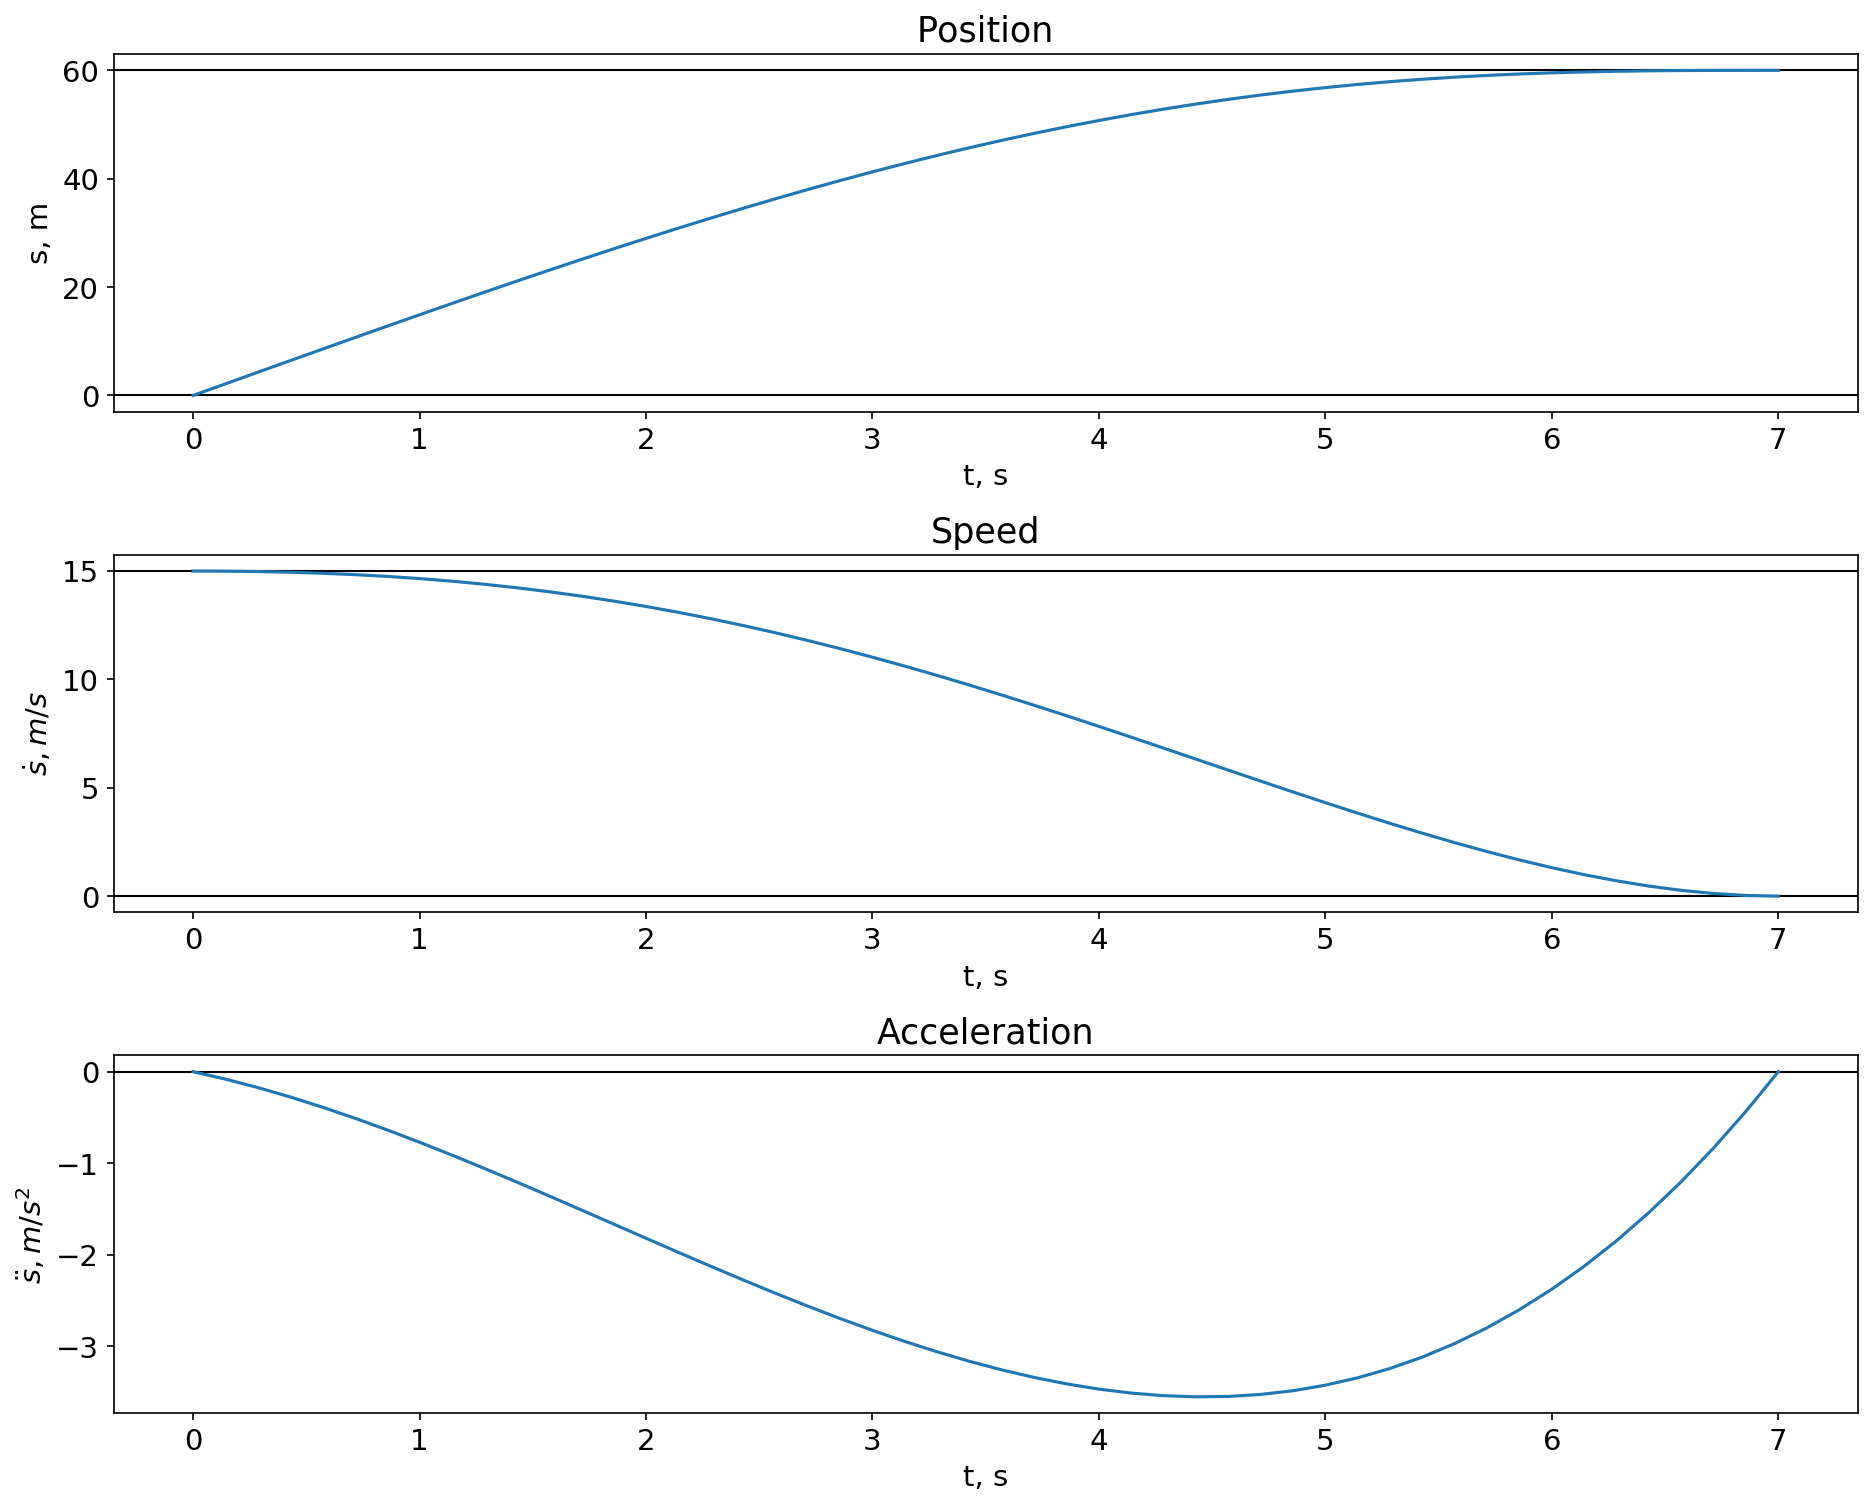
\includegraphics[width=\linewidth]{images/quintic_example}
      \caption{Пример траектории, описываемой полиномом пятого порядка}
      \label{img:quntic_example}
\end{figure}

Набор граничных условий, необходимый для формирования набора траекторий-кандидатов, формируется следующим образом.
Начальное продольное состояние:
\begin{equation}
      S_0 = <s_c, \dot{s}_c, 0>
\end{equation}
\noindent\begin{tabularx}{\linewidth}{lllX}
      где & $s_c$       &~---& текущее положение автомобиля вдоль опорной траектории, полученное от системы SLAM, \\
          & $\dot{s}_c$ &~---& текущая продольная скорость автомобиля, полученная от системы SLAM.
\end{tabularx}

Начальное поперечное состояние:
\begin{equation}
      D_0 = <d_c, \dot{d}_c, 0>
\end{equation}
\noindent\begin{tabularx}{\linewidth}{lllX}
      где & $d_c$       &~---& текущее поперечное отклонение автомобиля от опорной траектории , полученное от системы SLAM, \\
          & $\dot{d}_c$ &~---& скорость изменения поперечного отклонение, полученная от системы SLAM.
\end{tabularx}

Стоит заметить, что поперечная скорость $\dot{d}_c$ в общем случае не является скоростью бокового скольжения автомобиля
и может быть отличной от нуля даже в том случае, если автомобиль движется без бокового скольжения. Если вектор
продольной скорости автомобиля не параллелен касательной к опорной траектории, вектор продольной скорости будет разложен
в пару векторов $\dot{s}_c$ и $\dot{d}_c$.

Конечное продольное состояние:
\begin{equation}
      \begin{aligned}
            S_{1_{ij}} =& <s_i, v_j, 0> \\
            s_i =& s_1 + i\Delta s \\
            v_j =& \dot{s}_1 + i\Delta v
      \end{aligned}
\end{equation}
\noindent\begin{tabularx}{\linewidth}{lllX}
      где & $s_1$       &~---& требуемое положение автомобиля вдоль опорной траектории, получаемое от планировщиков высокого уровня, \\
          & $\dot{s}_1$ &~---& требуемая продольная скорость автомобиля, получаемая от планировщиков выского уровня, \\
          & $\Delta s$  &~---& шаг перебора продольных положений, \\
          & $\Delta v$  &~---& шаг перебора продольных скоростей.
\end{tabularx}

Конечное поперечное состояние:
\begin{equation}
      \begin{aligned}
            D_{1_{ij}} =& <d_i, 0, 0> \\
            d_i =& i\Delta d \\
      \end{aligned}
\end{equation}
\noindent\begin{tabularx}{\linewidth}{lllX}
      где & $\Delta d$  &~---& шаг перебора поперечных положений.
\end{tabularx}

Для перебора конечных состояний поперечных траекторий принимается, что требуемое поперечное положение (отклонение
автомобиля от опорной траектории) всегда равно нулю, т.е. автомобиль должен двигаться ровно по опорной траектории.
В том случае, когда это невозможно, в силу наличия препятствий, или существует более оптимальная траектория (например,
обгон медленно движущегося спереди автомобиля), поперечное движение автомобиля в пределах полосы или выход за ее пределы
осуществляется путем варьирования конечных поперечных состояний в локальном планировщике движения, а не за счет передачи
соответствующих целевых положений планировщиками движения более высокого уровня. Планировщик движения более
высокого уровня, такой как планировщик поведения, может дать команду на смену полосы движения, путем указания
новой опорной траектории, а требуемое  поперечное отклонение от новой траектории по прежнему будет нулевым.

Значения требуемых поперечных скоростей и ускорения полагаются всегда равными нулю, т.е. ожидается, что после завершения
маневра автомобиль будет двигаться параллельно опорной траектории.

Для расчета коэффициентов полинома, описывающего траекторию, требуется определение начального и конечного состояний, как
было описано выше. В качестве начального состояния принимается текущее состояние автомобиля, получаемое от системы
одновременной картографии и навигации (SLAM). Как было сказано выше, система SLAM, позволяет получить текущее положение
$<x, y, z>$ и ориентацию в виде кватерниона углов Эйлера $<\psi, \theta, \varphi>$
\noindent\begin{tabularx}{\linewidth}{lllX}
      где & $\psi$    &~---& рыскание (yaw), вращение вокруг оси $z$, \\
          & $\theta$  &~---& тангаж (pitch), вращение вокруг $y$, \\
          & $\varphi$ &~---& крен (roll), вращение вокруг оси $x$.
\end{tabularx}

Углы Эйлера и соответствующие оси изображены на рисунке \ref{img:euler_angles}.

\begin{figure}[h]
      \centering
      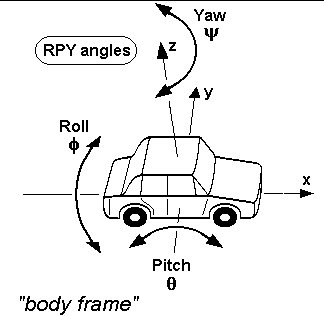
\includegraphics[width=0.5\linewidth]{images/euler_angles}
      \caption{Описание вращения с помощью углов Эйлера}
      \label{img:euler_angles}
\end{figure}

Таким образом, для автомобиля, движущегося на плоскости, состояние может быть задано следующим образом:
$<x, y, \psi, \dot{x}, \dot{y}, \dot{\psi}, \ddot{x}, \ddot{y}, \ddot{\psi}>$. Принимая, что боковое скольжение
отсутствует, состояние автомобиля можно записать в виде $<x, y, \psi, v, \dot{\psi}, a, \ddot{\psi}>$,
где $v$ ~--- продольная скорость, $a$ ~--- продольное ускорение.

Для применения рассматриваемого алгоритма планирования движения, требуется перевести состояние автомобиля из
глобальной декартовой системы координат в подвижную систему координат Френе. \hl{Написать про перевод, либо здесь,
либо в реализации}.

Помимо начального $<s_0, \dot{s}_0, \ddot{s}_0>$, и конечного $<s_1, \dot{s}_1, \ddot{s}_1>$ состояний, для расчета
коэффициентов полинома, согласно \ref{eq:solve_quintic} требуется задать требуемое время маневра $T$. С точки зрения
определения движения автомобиля, явное задание скорости, пройденного расстояния и требуемого для этого времени, является
избыточным. В большинстве случаев требуется монотонное изменение скорости автомобиля (например, ускорение или
замедление). Например, рассмотрим пример, приведенный на рисунке \ref{img:quntic_example}, где автомобиль
ормозит с начальной скорости 15 м/с до полной остановки за 7 секунд, преодолевая 60 метров. Для определения этой траектории
достаточно двух параметров: начальная скорость и требуемый тормозной путь позволяют рассчитать требуемое время, а
начальная скорость и требуемое время до полной остановки позволяют рассчитать требуемый тормозной путь. Существенное
превышение или уменьшение времени маневра $T$ по сравнению с необходимым для совершения этого маневра, не позволит
получить монотонную гладкую траекторию.

На рисунке \ref{img:quintic_bad_t} представлены три траектории:
голубая с близкой к оптимальной длительности маневра, оранжевая со слишком малой длительностью маневра и зеленая, со
слишком большой длительностью маневра. Видно, что при оптимальной длительности маневра положение автомобиля монотонно
возрастает, а скорость ~--- монотонно убывает. При слишком малой длительности маневра первоначально происходит
ускорение и лишь потом замедление до требуемой скорости. При слишком большой длительности маневра автомобиль сначала
проезжает мимо целевого положения, а затем возвращается, т.е. имеете место участок с отрицательной скоростью
(движение назад).

\begin{figure}[h]
      \centering
      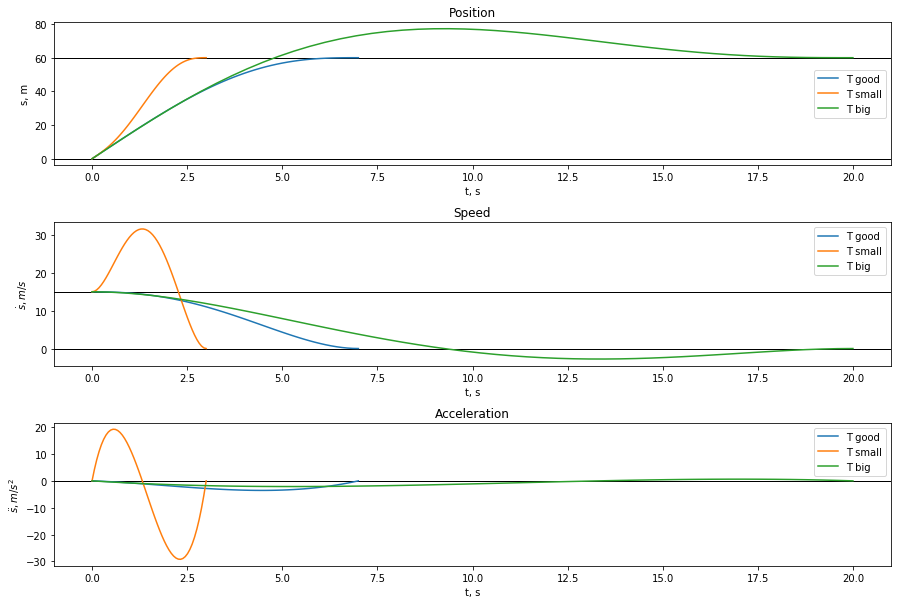
\includegraphics[width=\linewidth]{images/quintic_bad_t}
      \caption{Зависимость траектории от времени совершения маневра}
      \label{img:quintic_bad_t}
\end{figure}

Варьирование времени маневра $T$ может быть применено для получения различных профилей скорости. Так, например,
первоначальное ускорение с последующим замедлением может быть использовано при маневрах обгона.
В работе \cite{darpa_boss}, посвященной автомобилю "BOSS" Darpa Urban Challenge применяются несколько явно заданных
профилей скорости. С одной стороны, явное параметрическое задание профиля скорости позволяет более точно и задавать
требуемый профиль скорости и иметь большее число вариантов профиля скорости, в отличие от примененного в этой работе
метода, в котором профиль скорости задается неявно путем варьирования одного параметра ~--- длительности маневра $T$.
С другой стороны, метод, применяемый в автомобиле BOSS, обладает следующим недостатком: форма траектории и профиль
скорости выбираются независимо, в то время как в методе, реализуемым  в данной работе, профили скорости и ускорения
являются производными траектории, таким образом, этот метод лучше учитывает динамические характеристики автомобиля.

Таким образом, аналогично с варьированием конечных состояний, требуется варьировать длительность маневра:
\begin{equation}
      T_k = T_e + k\Delta T
\end{equation}
\noindent\begin{tabularx}{\linewidth}{lllX}
      где & $T_e$      &~---& начальная оценка длительности маневра, \\
          & $\Delta T$ &~---& шаг перебора длительностей маневра.
\end{tabularx}

Можно было бы задать в качестве начальной оценки заранее определенное константное значение времени либо перебирать
все значения от 0 до некого заданного $T_{max}$. Но это было бы неоптимально, потому что в таком случае было бы
сгенерировано большое количество траекторий со слишком малой или слишком большой длительностью маневра. Эти траектории
не повлияют на итоговый результат планирования движения, т.к. в любом случае будет выбираться оптимальная траектория,
минимизирующая функционал стоимости, но расчет большого количества избыточных траекторий серьезно увеличит вычислительные
затраты и время работы алгоритма.

Чтобы избежать этого был предложен метод приблизительной оценки требуемой длительности маневра $T_e$. В качестве оценки
требуемого времени совершения маневра принимается время совершения маневра с такими же начальными и конечными
условиями, но для случая равноускоренного движения:
\begin{equation}
      \begin{cases}
            \dot{s}_1 = \dot{s}_0 + aT_e \\
            s_1       = s_0       + \dot{s}_0T_e + \frac{aT_e^2}{2}
      \end{cases}
\end{equation}

Решая эту систему получим формулу расчет оценки времени маневра:
\begin{equation}
      T_e = 2\frac{s_0 - s_1}{\dot{s}_0 + \dot{s}_1}
\end{equation}

На рисунке \ref{img:quintic_t_estimate} приведен пример оценки длительности маневра. Пунктирная линия ~---
траектория равноускоренного движения, сплошные линии - траектории, полученные путем варьирования длительности
маневра при одинаковых начальных и конечных условиях. Данная оценка не является точной, потому что траектория движения
ищется в форме полиномов пятого порядка, соответственно, профиль скорости описывается полиномами четвертого порядка,
а предложенный метод оценивает необходимое время исходя о предположении о том, что ускорение неизменно и скорость
представлена в виде линейной функции. Тем не менее, эксперименты показали, что эта оценка подходит для практического
использования, т.к. после нахождения начального приближения длительности маневра формируется ряд траекторий-кандидатов
путем варьирования в том числе длительности маневра, из которых затем будет выбрана траектория, минимизирующая
функционал стоимости, поэтому даже если начальное приближение было не оптимальным, может быть выбрана более оптимальная
траектория. Варьирование длительности маневра создает при прочих неизменных параметрах создает набор
траекторий-кандидатов, отличающихся профилем скорости. Различные профили скорости играют роль при взаимодействии
с препятствиями, когда в результате совокупного влияния различных функционалов стоимости, оптимальный выбор может
отличаться от случая движения без помех, для которого оптимальным вариантом будет выбор траектории, наиболее
приближенной к начальной оценке. Для такого случая можно было бы дать точную оценку длительности маневра, которое
минимизирует функционал стоимости, но в более общем случае преимущества такой оценки сходят на нет. Преимуществом
предложенной оценки является ее крайне низкая вычислительная сложность, что немаловажно, т.к. в процессе планирования
движения требуется рассчитывать большое количество траекторий и осуществлять перепланирование как можно чаще.

\begin{figure}[h]
      \centering
      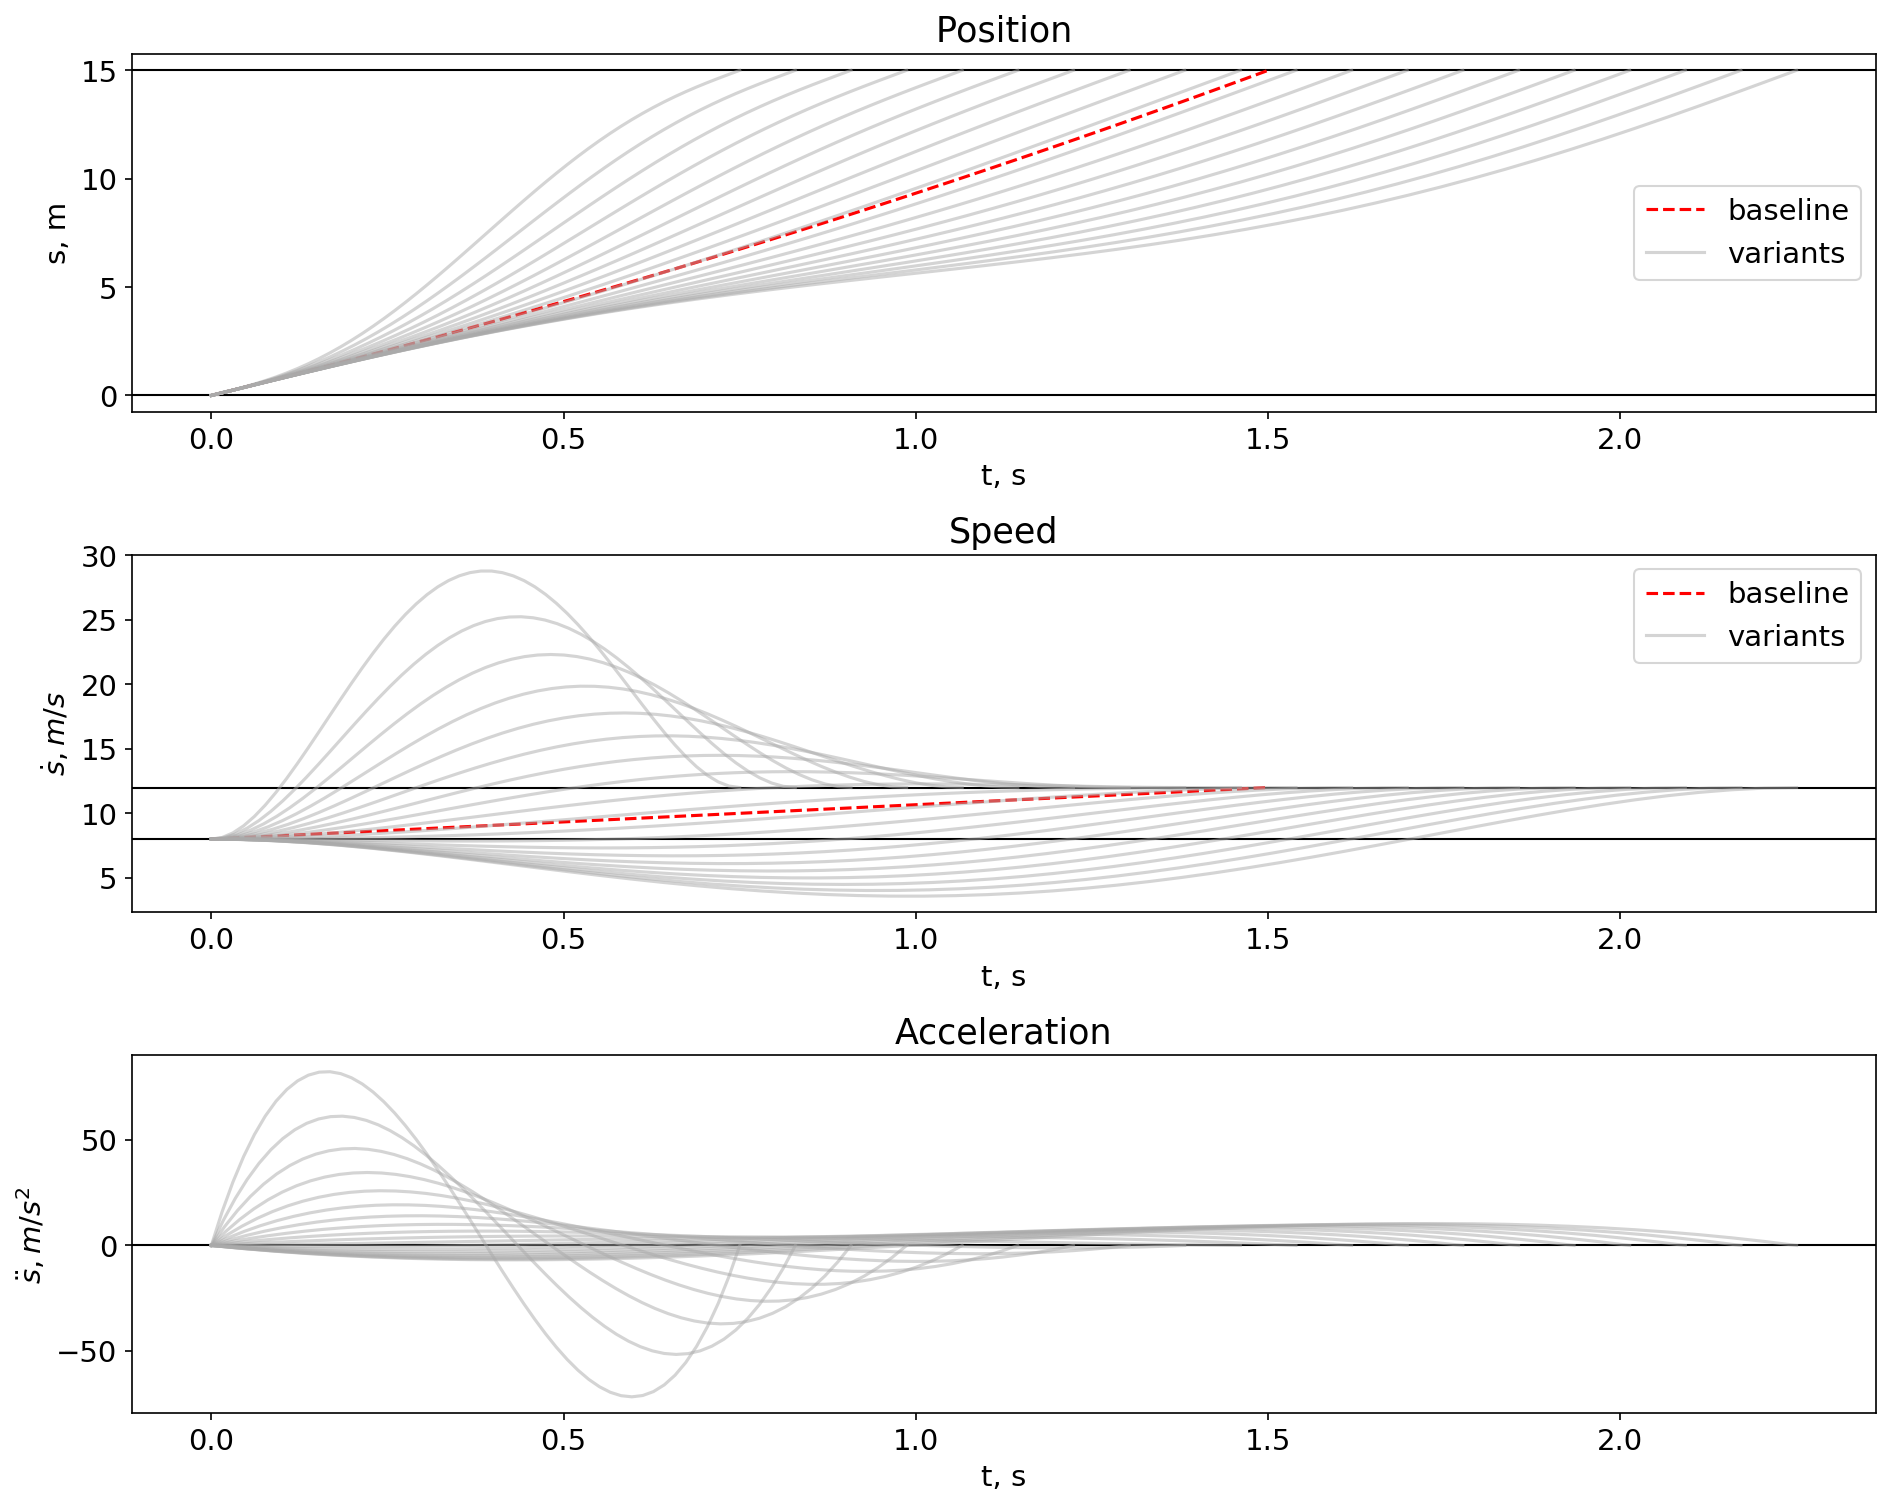
\includegraphics[width=\linewidth]{images/quintic_t_estimate}
      \caption{Пример оценки длительности маневра с помощью равноускоренного движения. Пунктирная линия ~---
      траектория равноускоренного движения, сплошные линии - траектории, полученные путем варьирования длительности
      маневра при одинаковых начальных и конечных условиях.}
      \label{img:quintic_t_estimate}
\end{figure}

Блок-схема рассмотренного алгоритма приведена на рисунке \ref{img:alg_quntic_planning_1}.

\begin{figure}[p]
      \centering
      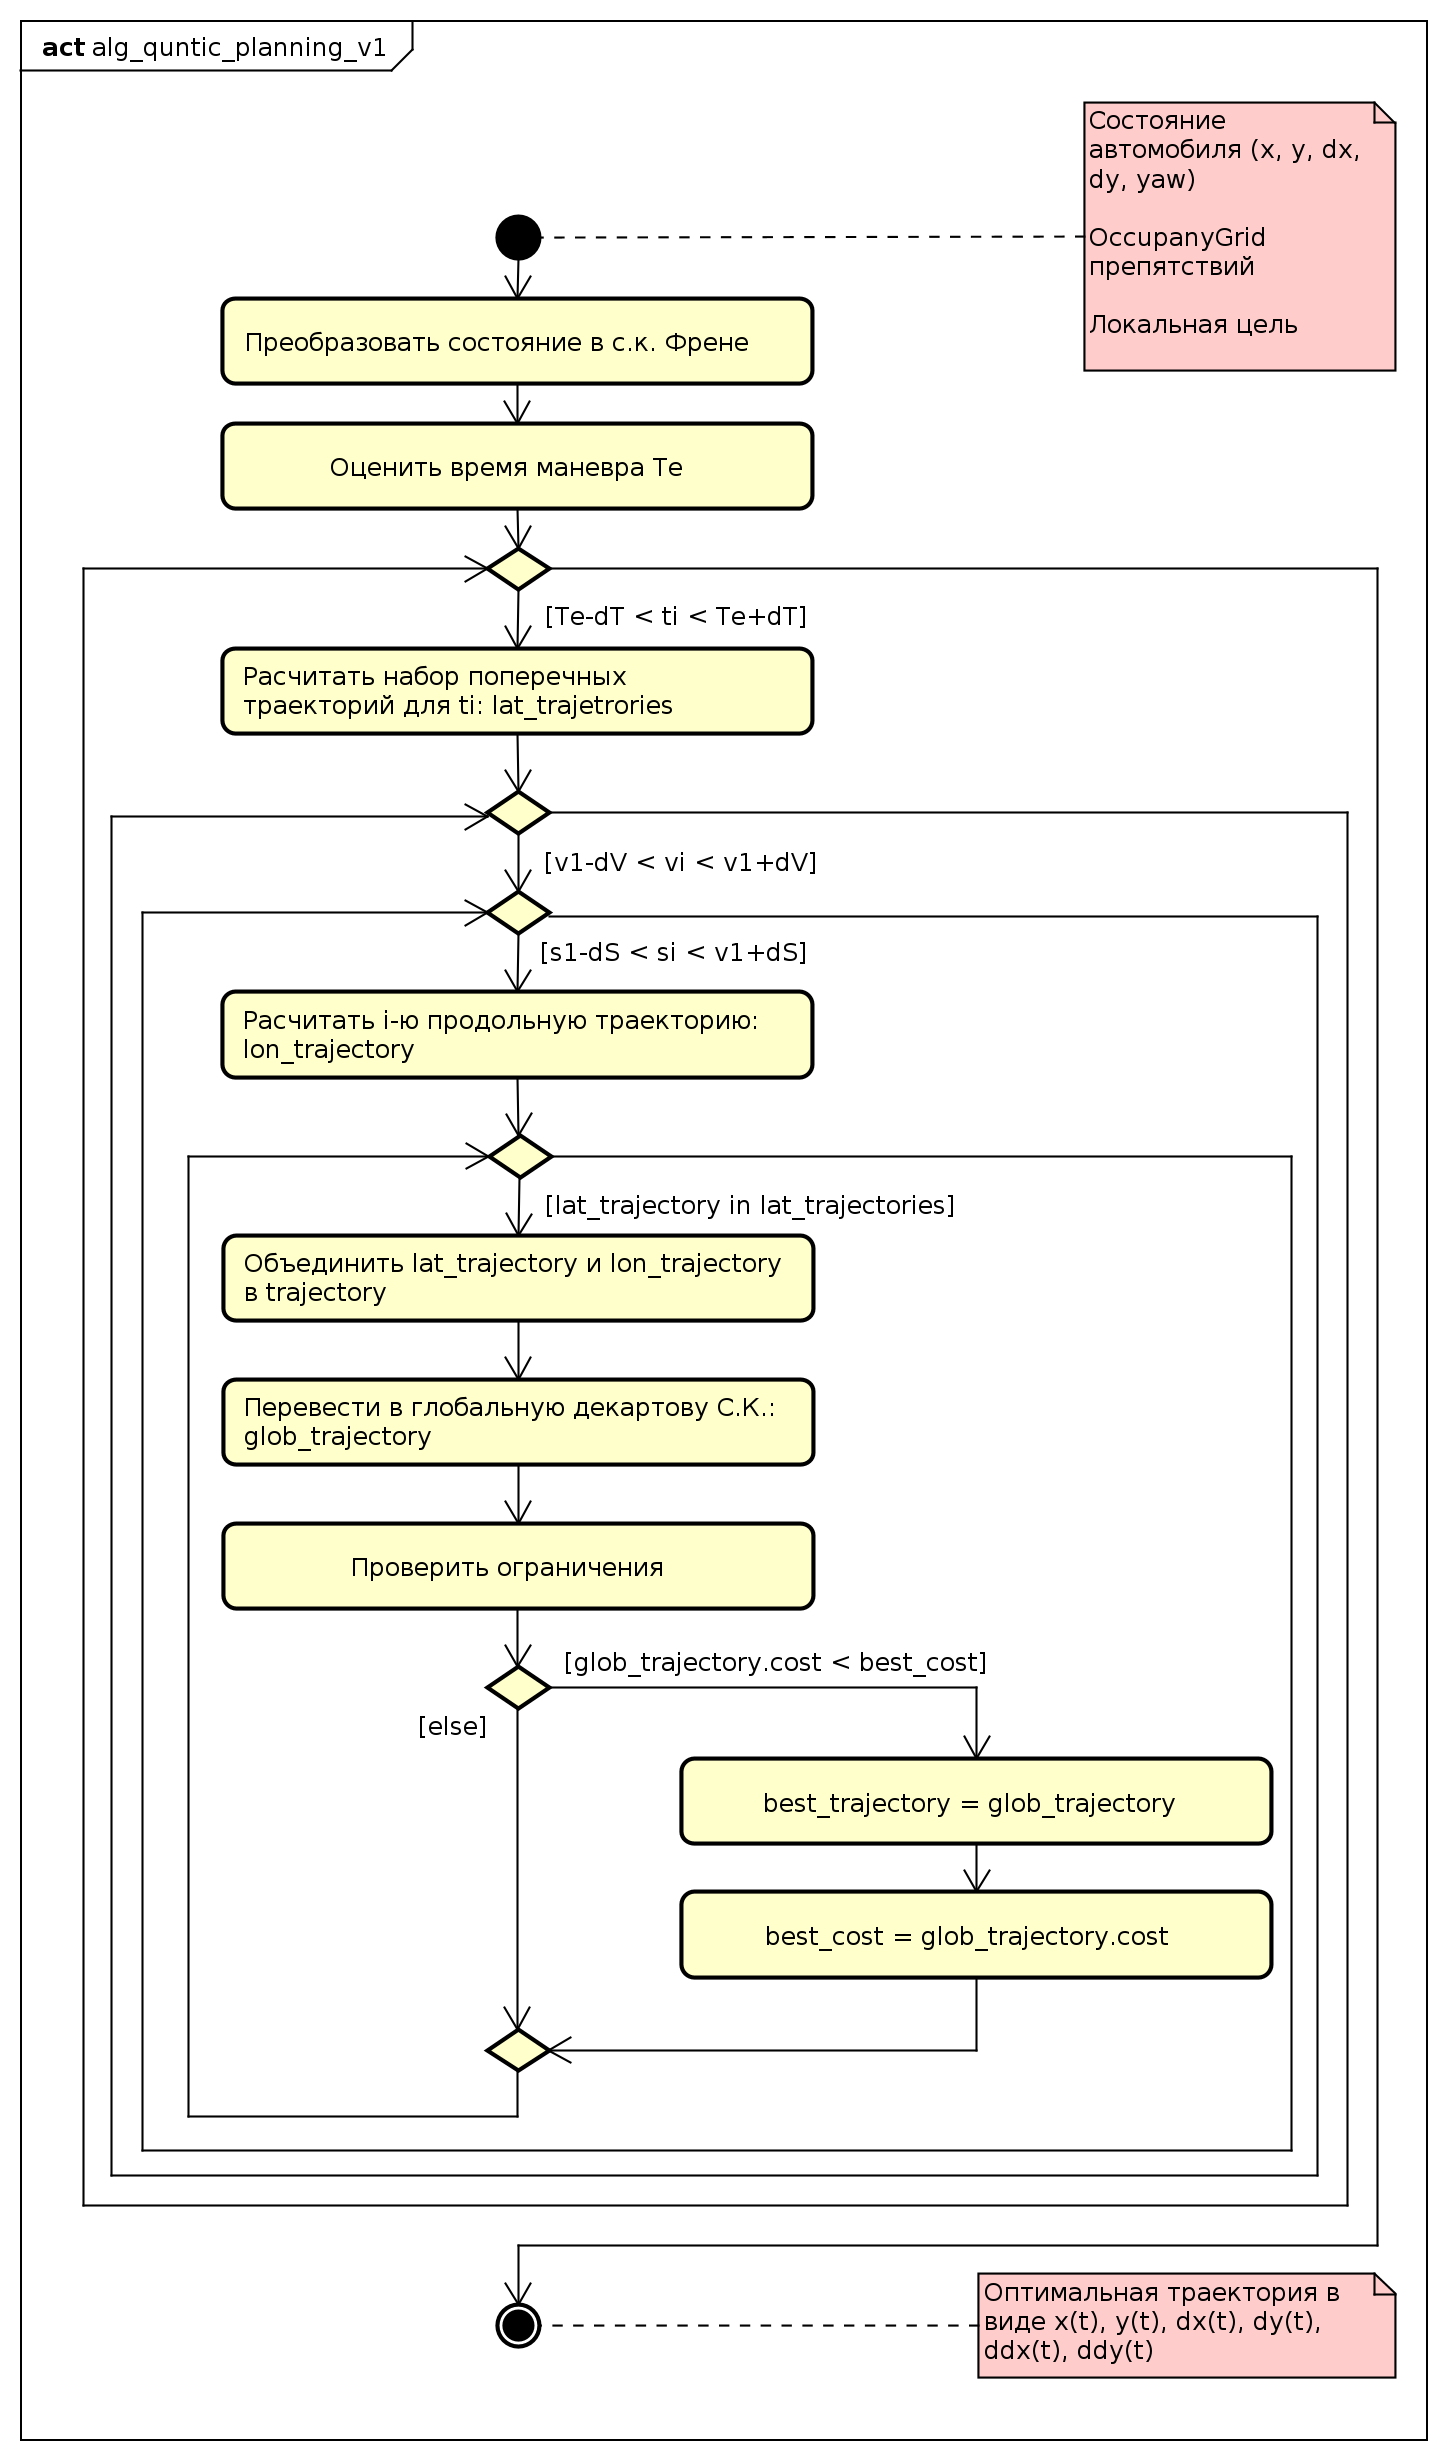
\includegraphics[height=0.95\textheight]{images/alg_quntic_planning_v1}
      \caption{Блок-схема алгоритма планирования движения}
      \label{img:alg_quntic_planning_1}
\end{figure}

На вход алгоритма подаются состояние автомобиля, полученное от системы SLAM, карта препятствий и локальная цель.
Вначале происходит преобразование начального состояния и целевого состояния в подвижную систему координат Френе,
заданную опорной траекторией. На основе заданных $s_0$, $\dot{s}_0$, $s_1$, $\dot{s}_1$, происходит расчет оценочного
времени маневра $T_e$.

Далее осуществляется переребор значение $t_i$, $s_i$ и $v_i$ во вложенных циклах. Для того, чтобы было возможно
совместить продольные и поперечные траектории необходимо, чтобы эти коэффициенты этих траекторий были рассчитаны для
одинаковой длительности маневра $ti$ и значения этих функций табулированы одинаковыми набором значений $t$.

Так как расчет продольных и поперечных траекторий независим, алгоритм можно оптимизировать, рассчитывая набор траекторий
один раз для каждого $t_i$, а затем объединяя их. Таким образом, на соответствующем шаге алгоритма для каждого $t_i$
генерируется и сохраняется набор поперечных траекторий, а затем для каждых $s_i$ и $v_i$ генерируется очередная
продольная траектория, которая объединяется со всеми предварительно рассчитанными поперечными траекториями.
Полученная траектория переводится обратно в глобальную систему координат и проверяется на удовлетворение ограничениям,
таким как минимальная кривизна и отсутствие пересечений с препятствиями.

%Алгоритм расчета набора поперечных траекторий для каждого $t_i$ представлен на рисунке
%\ref{img:alg_quintic_calc_lat_trajectories}. Алгоритм расчета продольной траектории аналогичен, за исключением отсутствия
%цикла, потому что он учтен в алгоритме верхнего уровня.

%\begin{figure}[h]
%      \centering
%      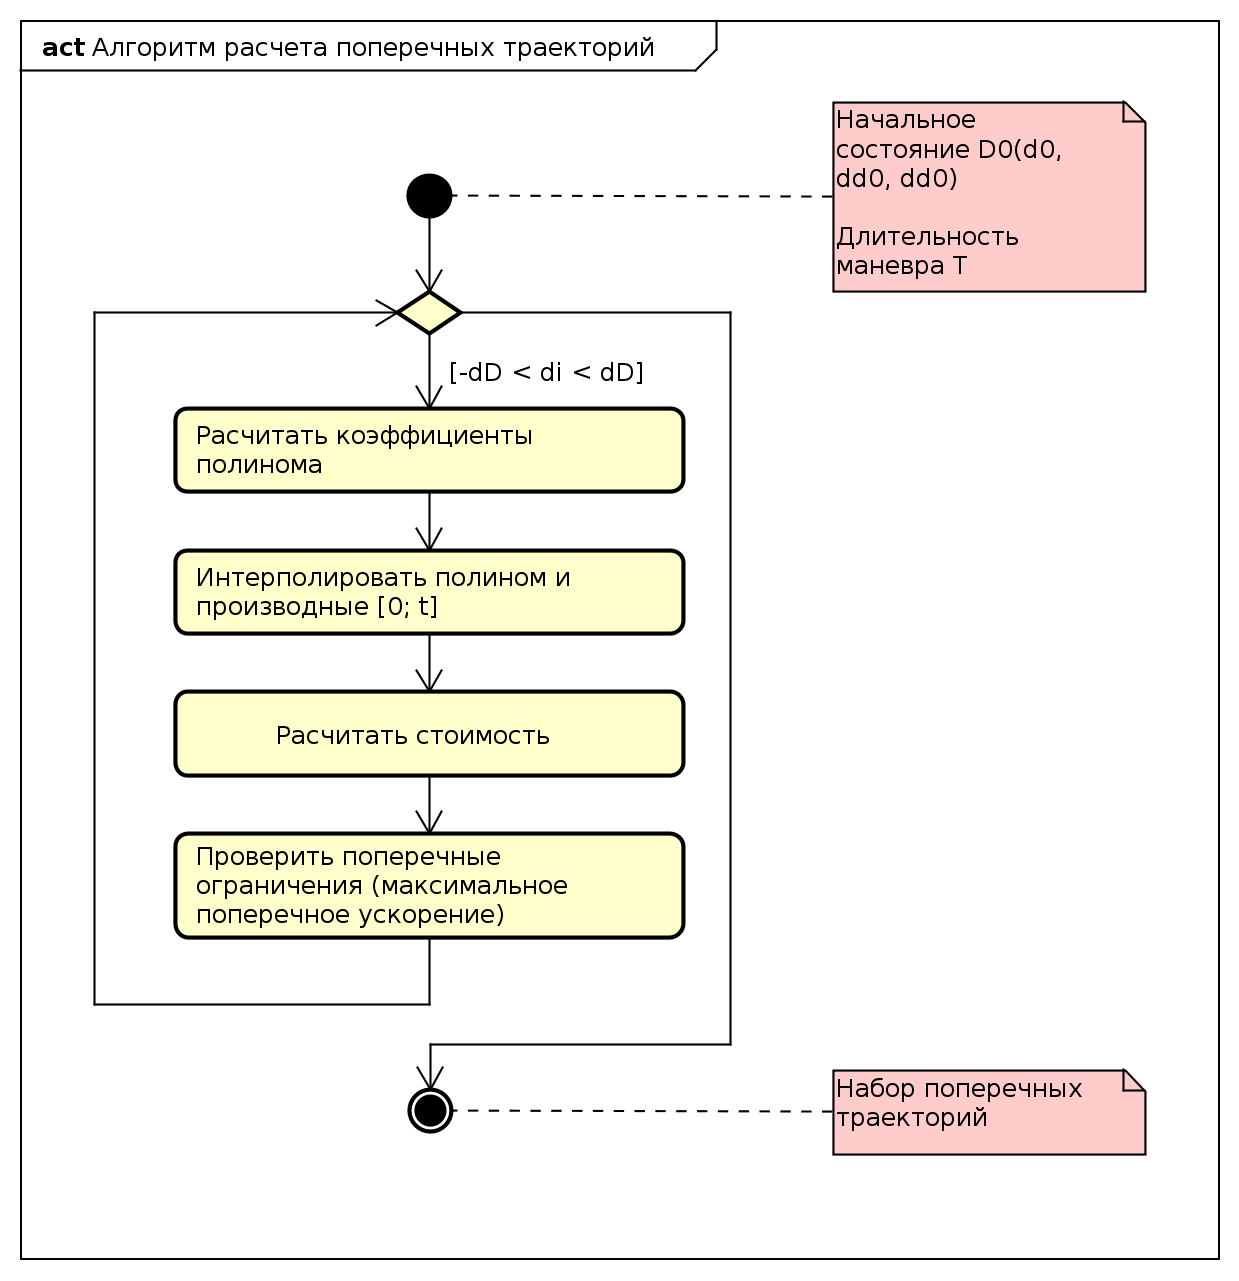
\includegraphics[width=0.7\linewidth]{images/alg_quintic_calc_lat_trajectories}
%      \caption{Блок-схема алгоритма расчета поперечных траекторий}
%      \label{img:alg_quintic_calc_lat_trajectories}
%\end{figure}

На рисунке \ref{img:quintic_results_1} представлен пример набора траекторий, сформированных алгоритмом путем варьирования
целевого продольного положения, целевого поперечного положения и длительности маневра. Параметры работы алгоритма выбраны
для большей наглядности полученного изображения, и отличаются от реальных параметров, которые необходимо использовать
при работе алгоритма. На рисунке представлены набор поперечных (слева) и продольных (справа) траекторий, включая их
первые и вторые производные, а также объединенные траектории. Цветом обозначается результат проверки ограничений.
Серым обозначены траектории, которые не удовлетворяют ограничениям, красным - траектории, которые удовлетворяют
ограничениям.

\begin{figure}[h]
      \centering
      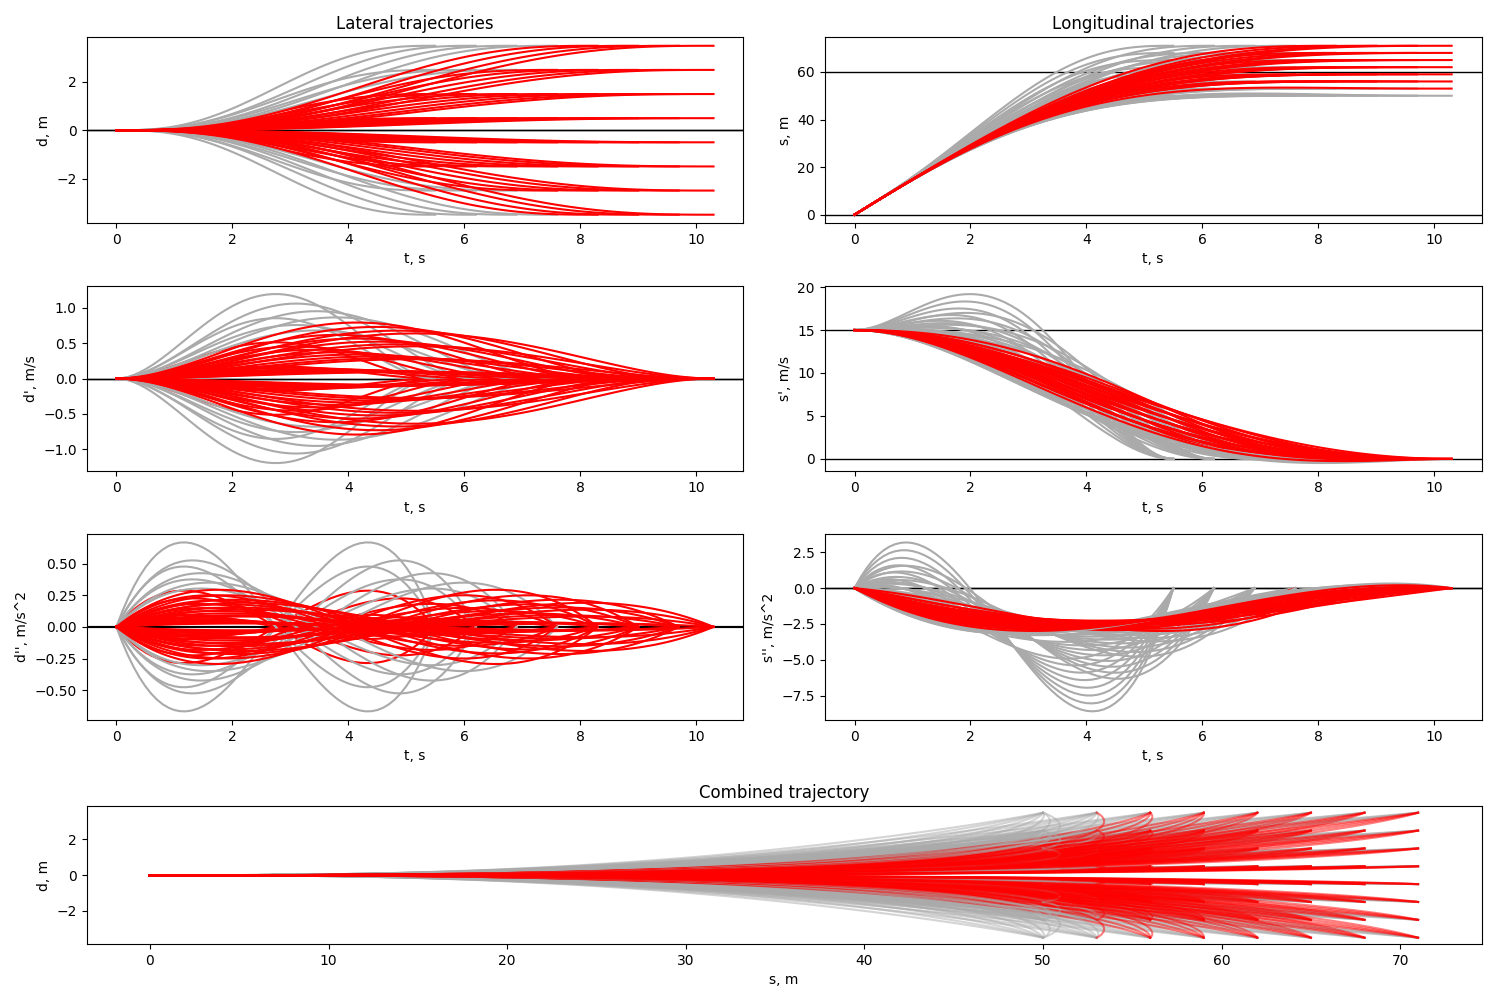
\includegraphics[width=\linewidth]{images/quintic_results_1}
      \caption{Пример формирования набора траекторий кандидатов. Серым обозначены траектории, которые не удовлетворяют
      ограничениям, красным - траектории, которые удовлетворяют ограничениям \hl{TODO: Что-то мутно как-то}}
      \label{img:quintic_results_1}
\end{figure}

%Разработанный алгоритм обладает рядом недостатков. Одним из недостатков является большое количество гиперпараметров,
%которые необходимо настроить. Алгоритм имеет следующие параметры:
%\begin{itemize}
%      \item $K_{dj}$, $K_d$, $K_{dt}$ ~--- весовые коэффициенты фунционала стоимости для поперечных траекторий;
%      \item $K_{sj}$, $K_s$, $K_v$, $K_st$ ~--- весовые коэффициенты функционала стоимости для продольных траекторий;
%      \item $D_{min}$, $D_{max}$, $\Delta D$ ~--- параметры перебора поперечных конечных состояний $d_i$,
%            минимальное, максимальное отклонение от от опорной траектории и шаг перебора состояний соответственно
%            (в силу того, что опорная траектория - центр полосы, $D_{min}=-D_{max}$);
%      \item $S_{min}$, $S_{max}$, $\Delta S$ ~--- параметры перебора продольных конечных состояний $s_i$;
%      \item $V_{min}$, $V_{max}$, $\Delta V$ ~--- параметры перебора продольных конечных скоростей $\dot{s}_i$;
%      \item $T_{min}$, $T_{max}$, $\Delta T$ ~--- параметры перебора длительности маневра.
% \end{itemize}
%В то время как параметры

\subsection{Планирование на несколько шагов}

Приведенный выше алгоритм был реализован и испытан на мобильной платформе с использованием обнаружения препятствий с
помощью LiDAR. Результаты испытания алгоритма показали, что алгоритм обладает недостатком, приводящим в определенных
ситуациях к тому, что он не может найти допустимую траекторию и автомобиль не может продолжать движение. Иллюстрация
такой ситуации приведена на рисунке \ref{img:quintic_planning_failed}.

\begin{figure}[h]
      \centering
      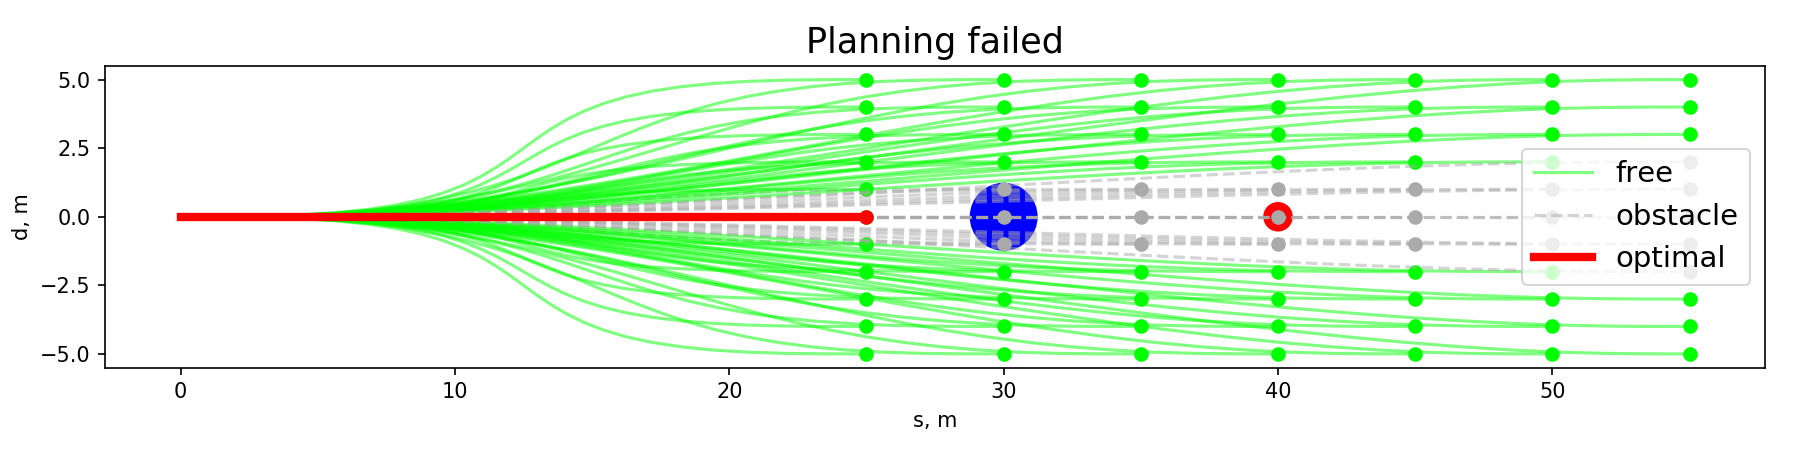
\includegraphics[width=\linewidth]{images/quintic_planning_failed}
      \caption{Пример планирования траектории с учетом препятствия при различных весовых коэффициентах.
      Подходящая траектория не была найдена (сверху), подходящая траектория была найдена (снизу).}
      \label{img:quintic_planning_failed}
\end{figure}

На рисунке изображена смоделированная ситуация. Автомобиль движется по дороге с постоянной скоростью, имеется локальная
цель с продольной координатой 40 м. Препятствие в форме окружности радиусом 1.5 м имеет продольную координату 30 м.
Для наглядности изображения осуществлялось варьирование только продольных и поперечных координат конечного состояния,
скорость и время маневра не изменялись. На рисунке изображены два результата планирования с различными весовыми
коэффициентами в функционале стоимости.

Для того, чтобы объехать препятствие, автомобиль должен отклониться от опорной траектории. Этот маневр приведет
к следующим изменениям в функционале стоимости \ref{eq:cost_lon}:
\begin{itemize}
      \item отклонение $d$ от опорной траектории увеличиться, что приведет к увеличению члена $K_dd(T)^2$;
      \item совершенные маневры приведут к увеличению $K_{dj}\int_{t_0}^{t_1}{\dddot{s}(t)^2dt}$;
      \item общее время маневра приведет к увеличению члена $K_{st}T$;
      \item автомобиль будет ближе к продольной цели, что приведет к уменьшению $K_s(s(T)-S_1)^2$
\end{itemize}

Итоговое значение функционала стоимости и принятое решение зависит от соотношения весовых коэффициентов $K_d$, $K_{dj}$,
$K_{st}$, $K_s$.

Эту проблему можно решить, если модифицировать алгоритм планирования движения путем осуществления нескольких шагов
планирования, т.е. рекурсивно запустить планирование повторно из каждого конечного состояния. Такой метод существенно
увеличит вычислительную сложность алгоритма, но позволит осуществлять планирование с большим горизонтом и осуществлять
более сложные маневры.

Для реализации этого алгоритма было решено совместить рассмотренный выше алгоритм с механизмом решетки состояний
(state lattice) \cite{motion_planning_lattice_1}. Как было рассмотрено в первой главе, эквивалентные траектории
можно представить в виде последовательности элементарных траекторий. В данном случае, требуется заменить рекурсивный
вызов планирования из каждой конечной точки построением графа, куда каждая начальная и конечная точка входит только один
раз. Дело в том, что из-за того, что конечные состояния представлены в виде регулярной решетки, попасть в некое
конечное состояние можно несколькими способами, и осуществлять планирование отрезка траектории, начинающегося из
этого состояния несколько раз не требуется. Это позволит существенно уменьшить вычислительную сложность алгоритма.

Помимо реализации планирования на несколько шагов в вперед, в алгоритм добавлена еще одна модификация. В предыдущей
версии алгоритма оценка длительности времени маневра осуществляется на основе целевого положения, а затем используется
при всех перебираемых значения конечного положения и скорости. В новой версии алгоритма оценка времени осуществляется
для каждой пары начальное состояние-конечное состояние. Сравнение двух методов формирования траекторий приведено
на рисунке \ref{img:t_estimate_compare}. При оценке времени маневра для каждой пары состояний, все полученные
траектории удовлетворяют требованию монотонности, т.е. в рассматриваемом примере торможения автомобиля не происходит
ни ускорений, ни возврата назад, как это происходит в первом варианте. Для получения различных профилей скорости,
применяется варьирование длительности маневра уже после оценки.

\begin{figure}[h!]
      \begin{minipage}[h]{0.49\linewidth}
            \center{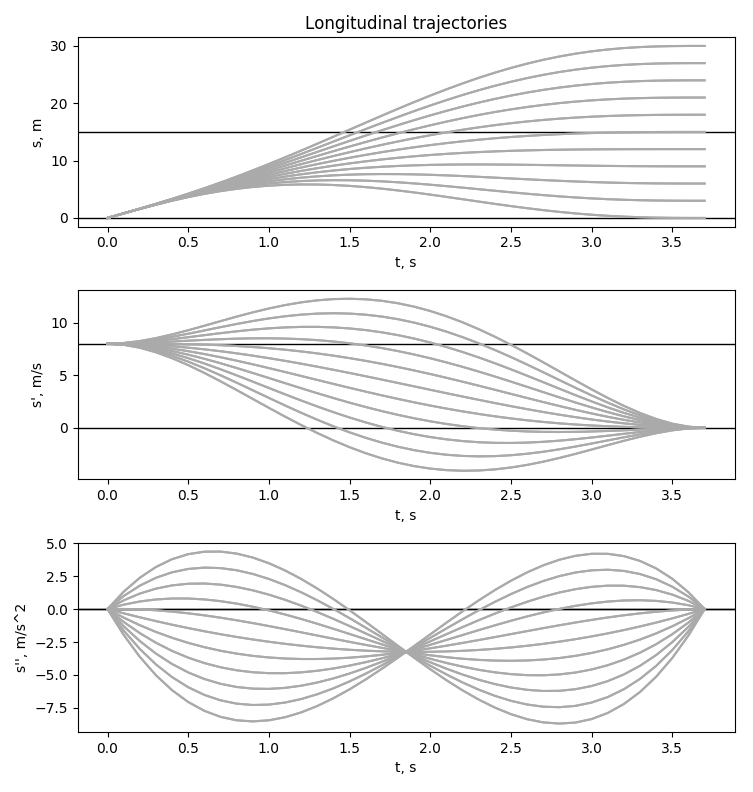
\includegraphics[width=\linewidth]{images/2_project/quintic_2/t_estimate_one_time} \\ а)}
      \end{minipage}
      \hfill
      \begin{minipage}[h]{0.49\linewidth}
            \center{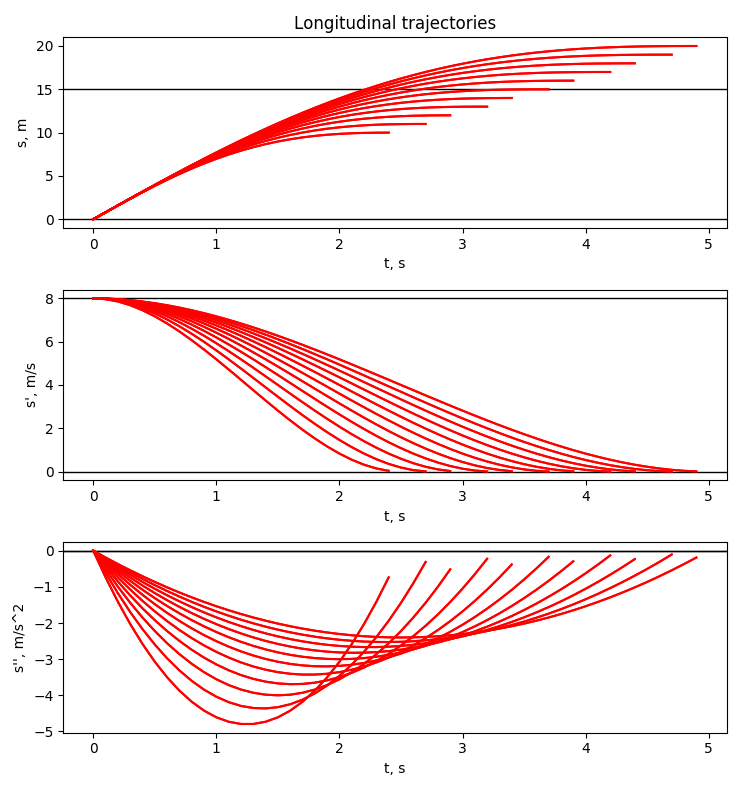
\includegraphics[width=\linewidth]{images/2_project/quintic_2/t_estimate_multiple} \\ б)}
      \end{minipage}
      \caption{Сравнение получаемых траекторий при оценке времени: а) при оценке времени один раз на основе цели,
      б) при оценке времени для каждой пары "начальное состояние-конечное состояние"}
      \label{img:t_estimate_compare}
\end{figure}

Планирование траекторий осуществляется путем построения графа возможных траекторий и нахождении оптимальной траектории
с помощью алгоритма Дейкстры.

Алгоритм Дейкстры является хорошо известным алгоритмом, для решения т.н. задачи "Single-source Shortest Path", т.е.
нахождение кратчайших путей на графе до всех вершин от заданной. В отличие от этой задачи, в задаче планирования
движения требуется не только найти кратчайший путь на графе, но и выбрать конечную вершину, которая даст оптимальную
траекторию движения. Исходя из функционала стоимости \ref{eq:cost_tot}, применяемого для оценки траекторий кандидатов,
можно сказать, что оценка траектории складывается из двух компонент: стоимости траектории, определяемой резкостью
совершаемых маневров, и стоимостью конечного состояния, определяемого его удаленности от цели. С учетом этого, можно
переписать функционал стоимости следующим образом, просто перегруппировав члены и разделив его на функционал стоимости
движения и функционал стоимости
состояния:

\begin{align}
      C_{move}  = &K_{lon}K_{sj}\int_{0}^{T}{\dddot{s}(t)^2dt} + K_{lat}K_{dj}\int_{0}^{T}{\dddot{d}(t)^2dt} \\
      C_{state} = &K_{lon}\Big[K_s \big(s(T) - S_1\big)^2 + K_v \big(\dot{s}(T) - \dot{S_1}\big)^2 + K_{st} T\Big] + \\
                  &K_{lat}\Big[K_d d(T)^2 + K_{dt} T\Big] \nonumber
\end{align}

Алгоритм планирования движения состоит из трех стадий: на первой осуществляется построение графа
состояний с расчетом траекторий, являющихся ребрами, на второй осуществляется нахождением минимальной стоимости движения
(т.е. учитывается только резкость маневров) до каждого конечного состояния с помощью алгоритма Дейкстры, на третьей
осуществляется выбор оптимального конечного состояния с учетом стоимости движения и его удаленности от цели.

Блок-схема формирования набора траекторий приведена на рисунке \ref{img:alg_create_graph}.

\begin{figure}[h!]
      \begin{minipage}[b]{0.49\linewidth}
            \center{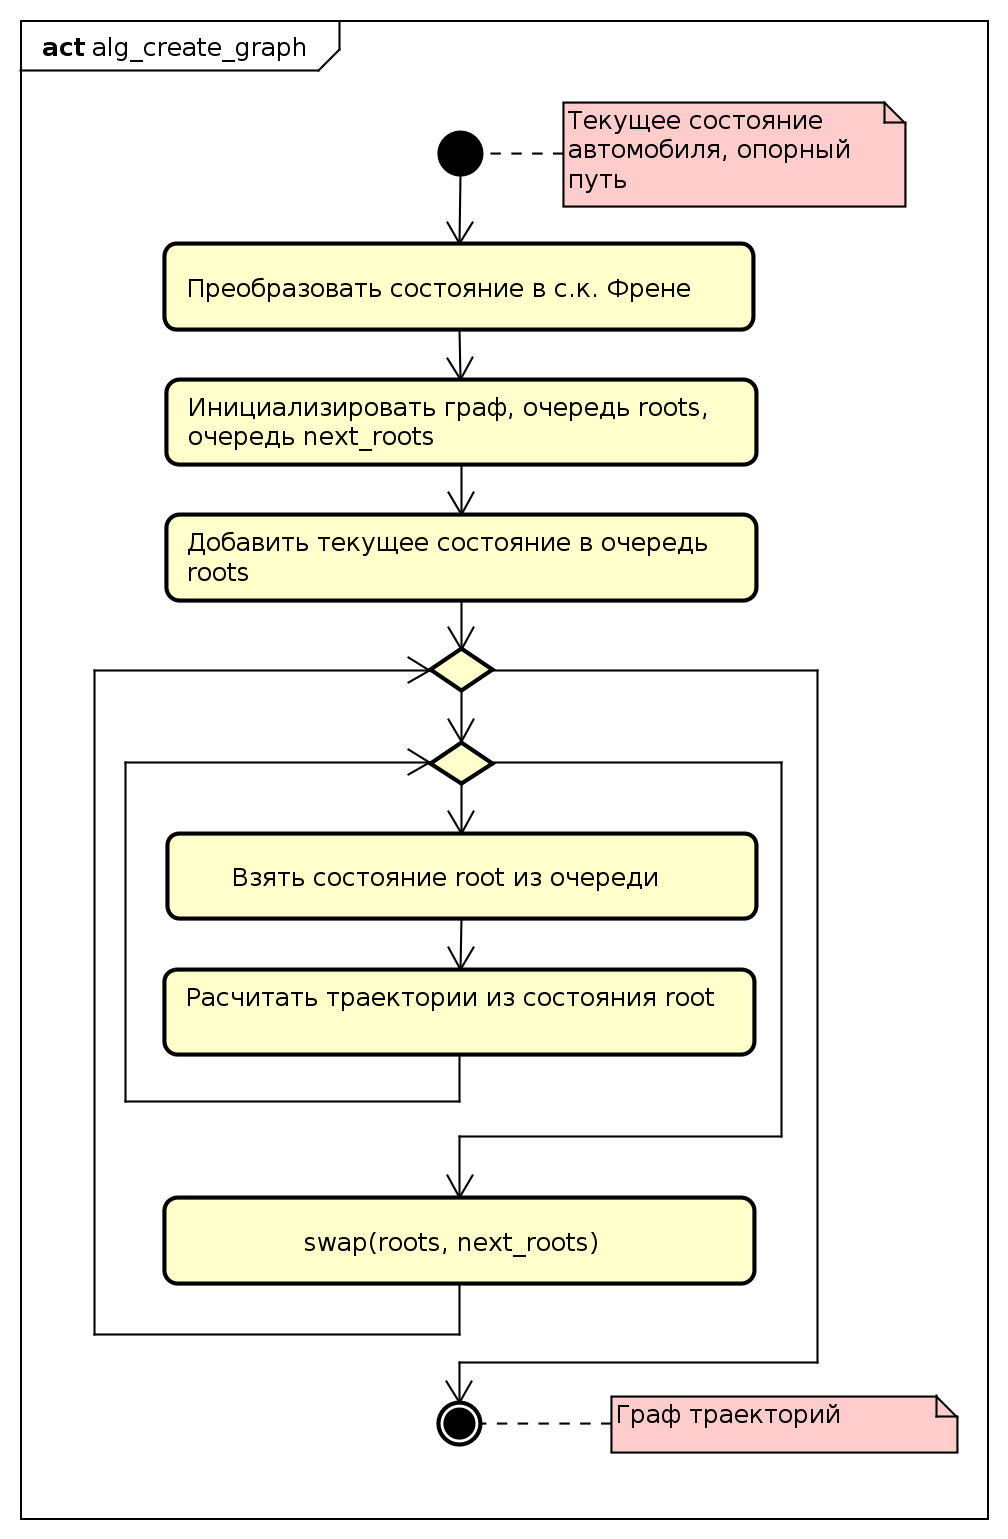
\includegraphics[width=\linewidth]{images/2_project/quintic_2/alg_create_graph} \\ а)}
      \end{minipage}
      \hfill
      \begin{minipage}[b]{0.49\linewidth}
            \center{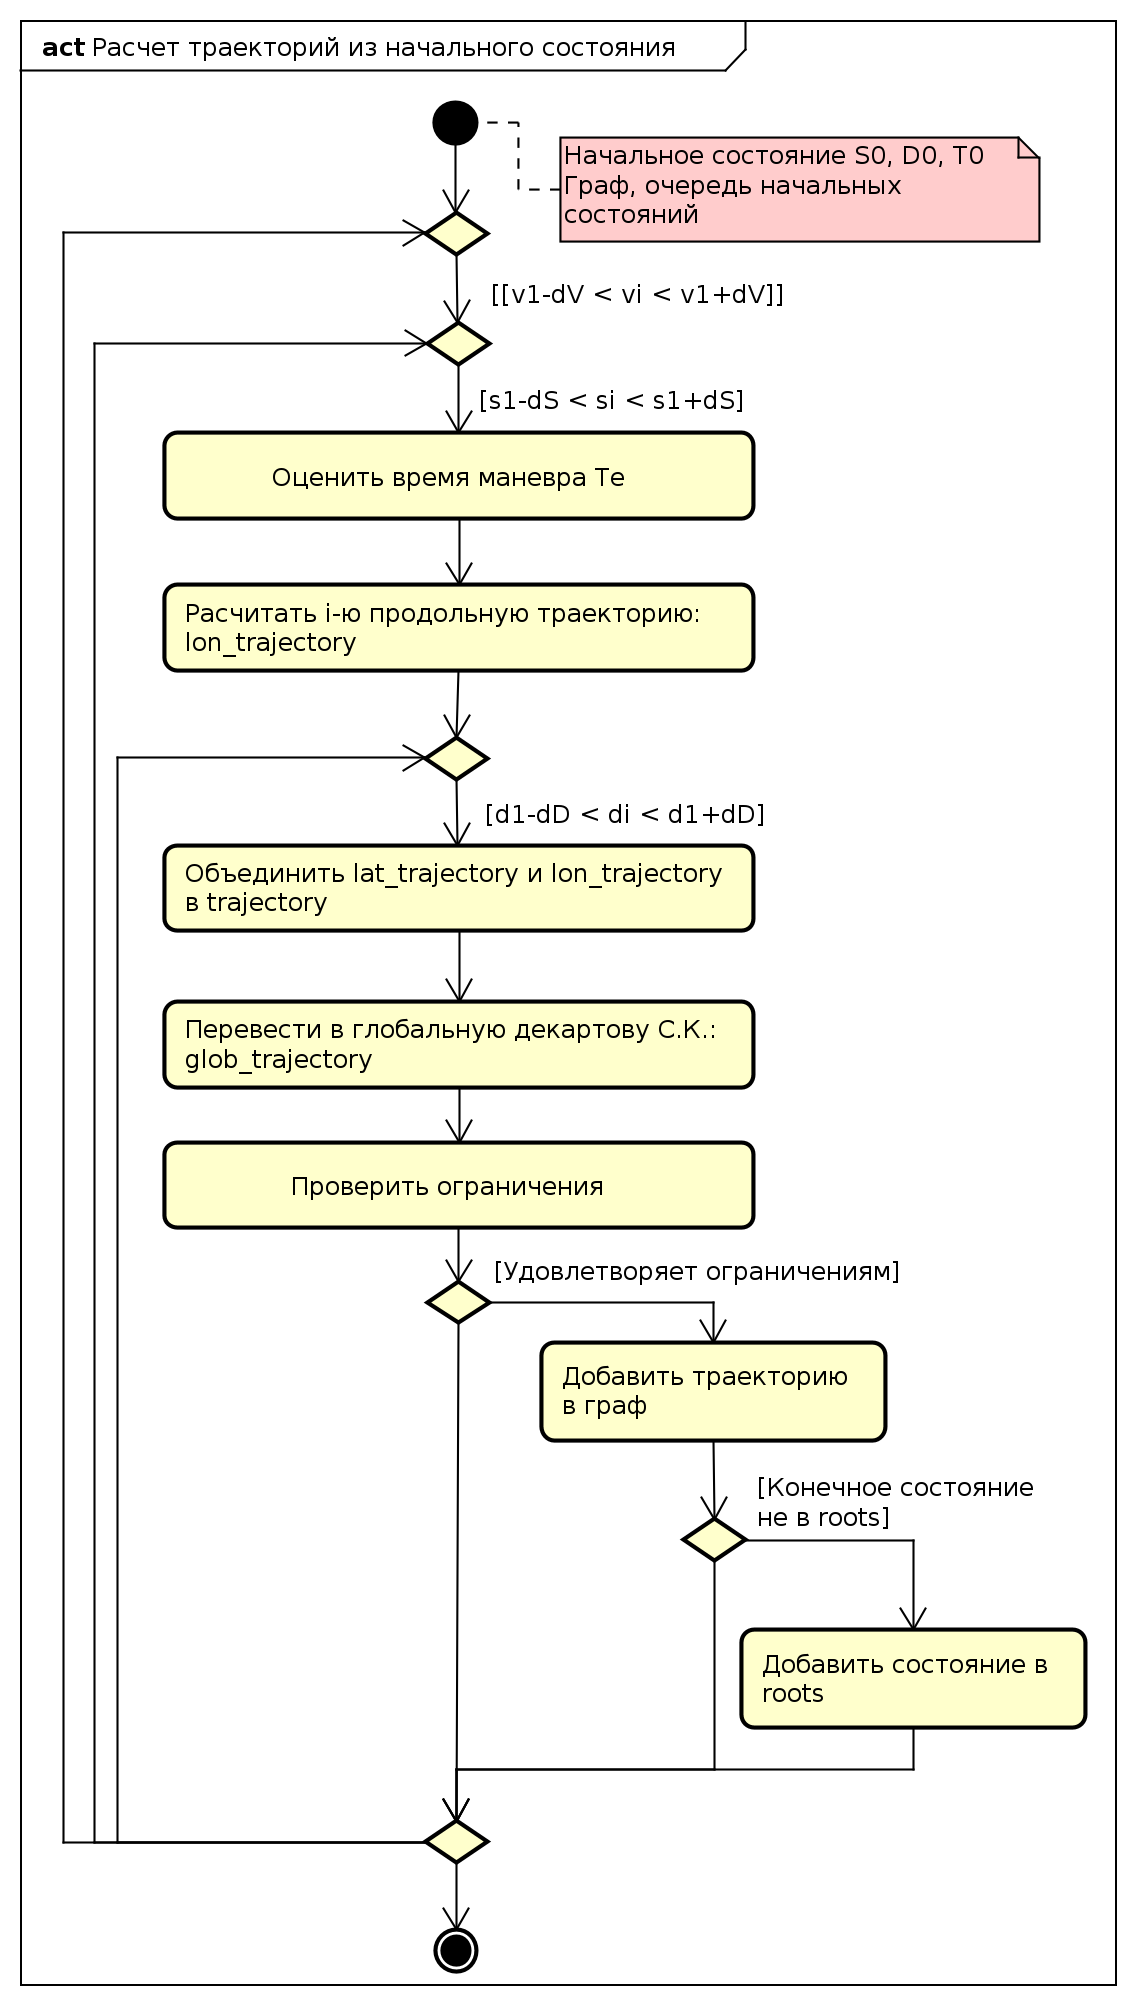
\includegraphics[width=\linewidth]{images/2_project/quintic_2/alg_create_trajectories_from_root} \\б)}
      \end{minipage}
      \caption{а) блок-схема алгоритма построения графа, б) блок схема шага расчета набора траекторий из заданного
      начального состояния. }
      \label{img:alg_create_graph}
\end{figure}

На вход подаются состояние автомобиля, полученное от системы SLAM, карта препятствий и локальная цель. Вначале
происходит преобразование начального состояния и целевого состояния в подвижную систему координат Френе, заданную
опорной траекторией. Инициализируются пустой граф и две пустых очереди для хранения новых состояний, из которых
для которых осуществляется формирование траекторий. В качестве первого начального состояния в очередь помещается
текущее состояние автомобиля в системе координат Френе. Алгоритм работает до тех пор, пока не будет построено
необходимое количество слоев графа. При заполнении каждого слоя из очереди извлекается очередное состояние и
осуществляется формирование набора траекторий, начинающихся из этого состояний. Конечные состояния этих траекторий
помещаются в очередь, чтобы быть использованы для формирования нового слоя. В алгоритме используется две очереди
состояний, которые переключются после заполнения каждого слоя. Это сделано потому что в случае применения одной очереди,
она бы постоянно пополнялась в процессе расчета траекторий. В данном случае, когда одна очередь становится пустой, это
означает, что из всех состояний текущего слоя были построены траектории, и происходит переключение на другую очередь,
которая хранит начальные состояния для другого слоя.

Следующим этапом алгоритма планирования траектории является нахождение кратчайших путей до всех вершин с помощью
алгоритма Дейкстры. Блок схема алгоритма изображена на рисунке \ref{img:alg_dijkstra}.

\begin{figure}[h]
      \centering
      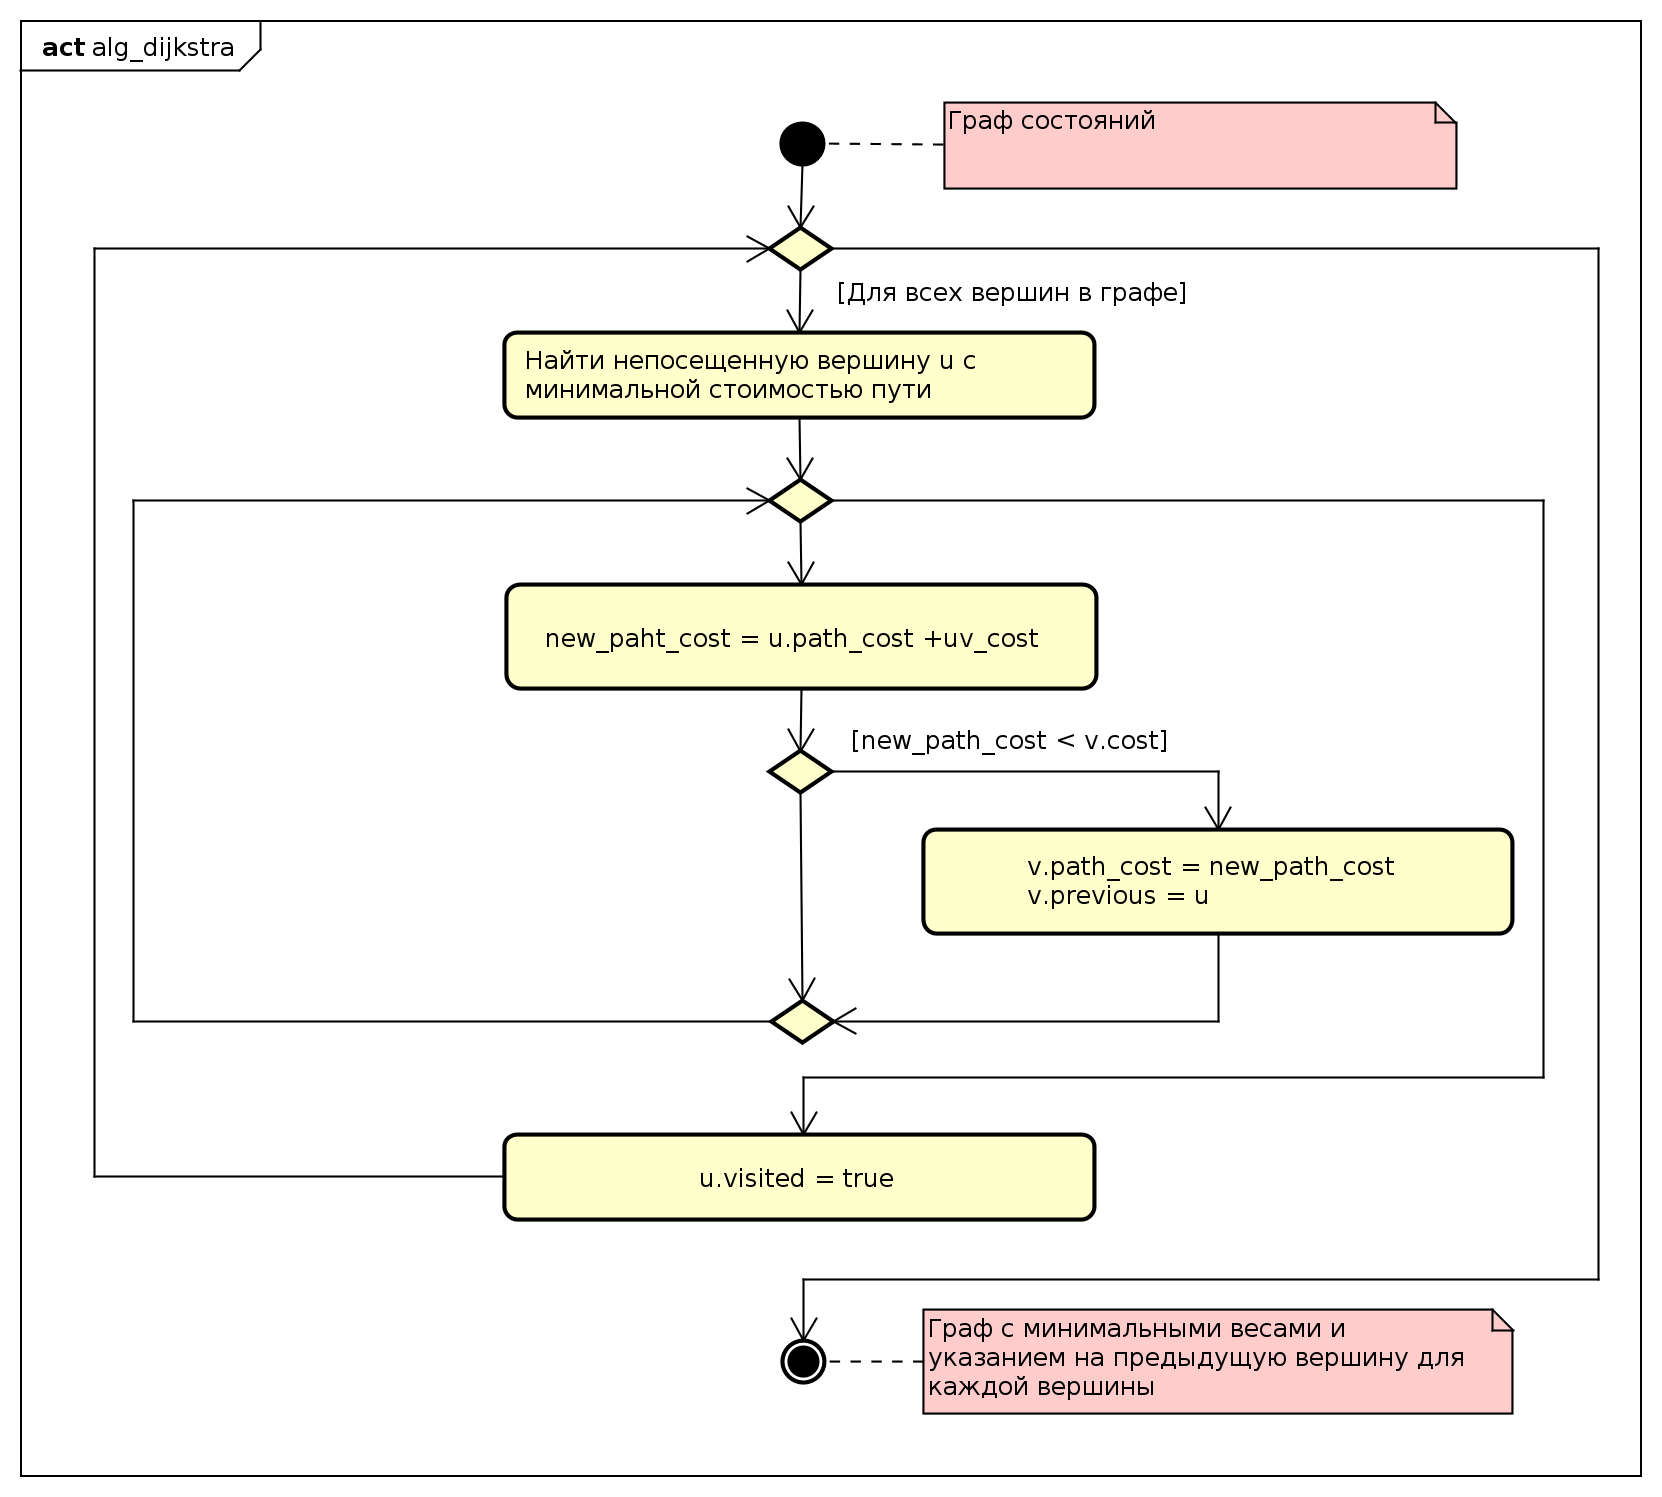
\includegraphics[width=\linewidth]{images/2_project/quintic_2/alg_dijkstra}
      \caption{Алгоритм Дейкстры}
      \label{img:alg_dijkstra}
\end{figure}

Вначале алгоритма стоимость пути до всех путей, кроме начальной, инициилизируется равной бесконечности. Все вершины
отмечаются, как непосещенные.
Алгоритм Дейкстры состоит из количества итераций, равному количеству вершин в графе. На каждой итерации алгоритма
выбирается вершина $u$ с минимальной стоимостью пути из начальной до нее. Это может быть сделано
простым перебором за $O(N)$, использование различных структур данных может сократить асимптотическую оценку, например,
использование двоичной кучи позволяет находить вершину за $O(logN)$. Более того, за счет того, что граф
имеет регулярную структур и проходится слой за слоем, можно ограничить диапазон поиска вершины с минимальной стоимостью
ути. Затем перебираются все вершины $v$, связанные ребром с $u$. Рассчитывается, какая стоимость пути будет до вершин $v$,
если двигаться к ней через вершину $u$: $new\_path\_cost = u.path\_cost + uv\_edge\_cost$, и если эта стоимость меньше,
чем та, которая сохранена в вершине $v$, значение стоимости пути до вершины $v$ обновляется. Для того, чтобы в дальнейшем
можно было восстановить кратчайший маршрут, а не только получить его стоимость, для вершины $v$ обновляется предыдущая
вершина кратчайшего маршрута ~--- вершина $v$. После обработки всех связанных вершин, вершина $u$ отмечается как
посещенная, и после этого алгоритм переходит к следующей итерации.

Финальным этапом алгоритма является выбор оптимального конечного состояния, которое обладает минимальным суммарным
весом $C = C_{move} + C_{state}$, где $C_{move}$ получен в результате алгоритма Дейкстры, а $C_{move}$ для каждой
вершины рассчитан при формировании графа.

% Можно было бы и этот алгоритм нарисовать, но я что-то очень устал это делать

Пример формирования набора траекторий представлен на рисунке \ref{img:multistep_trajectories}. Для наглядности
осуществлялось варьирование только поперечных конечных состояний.

\begin{figure}[h]
      \centering
      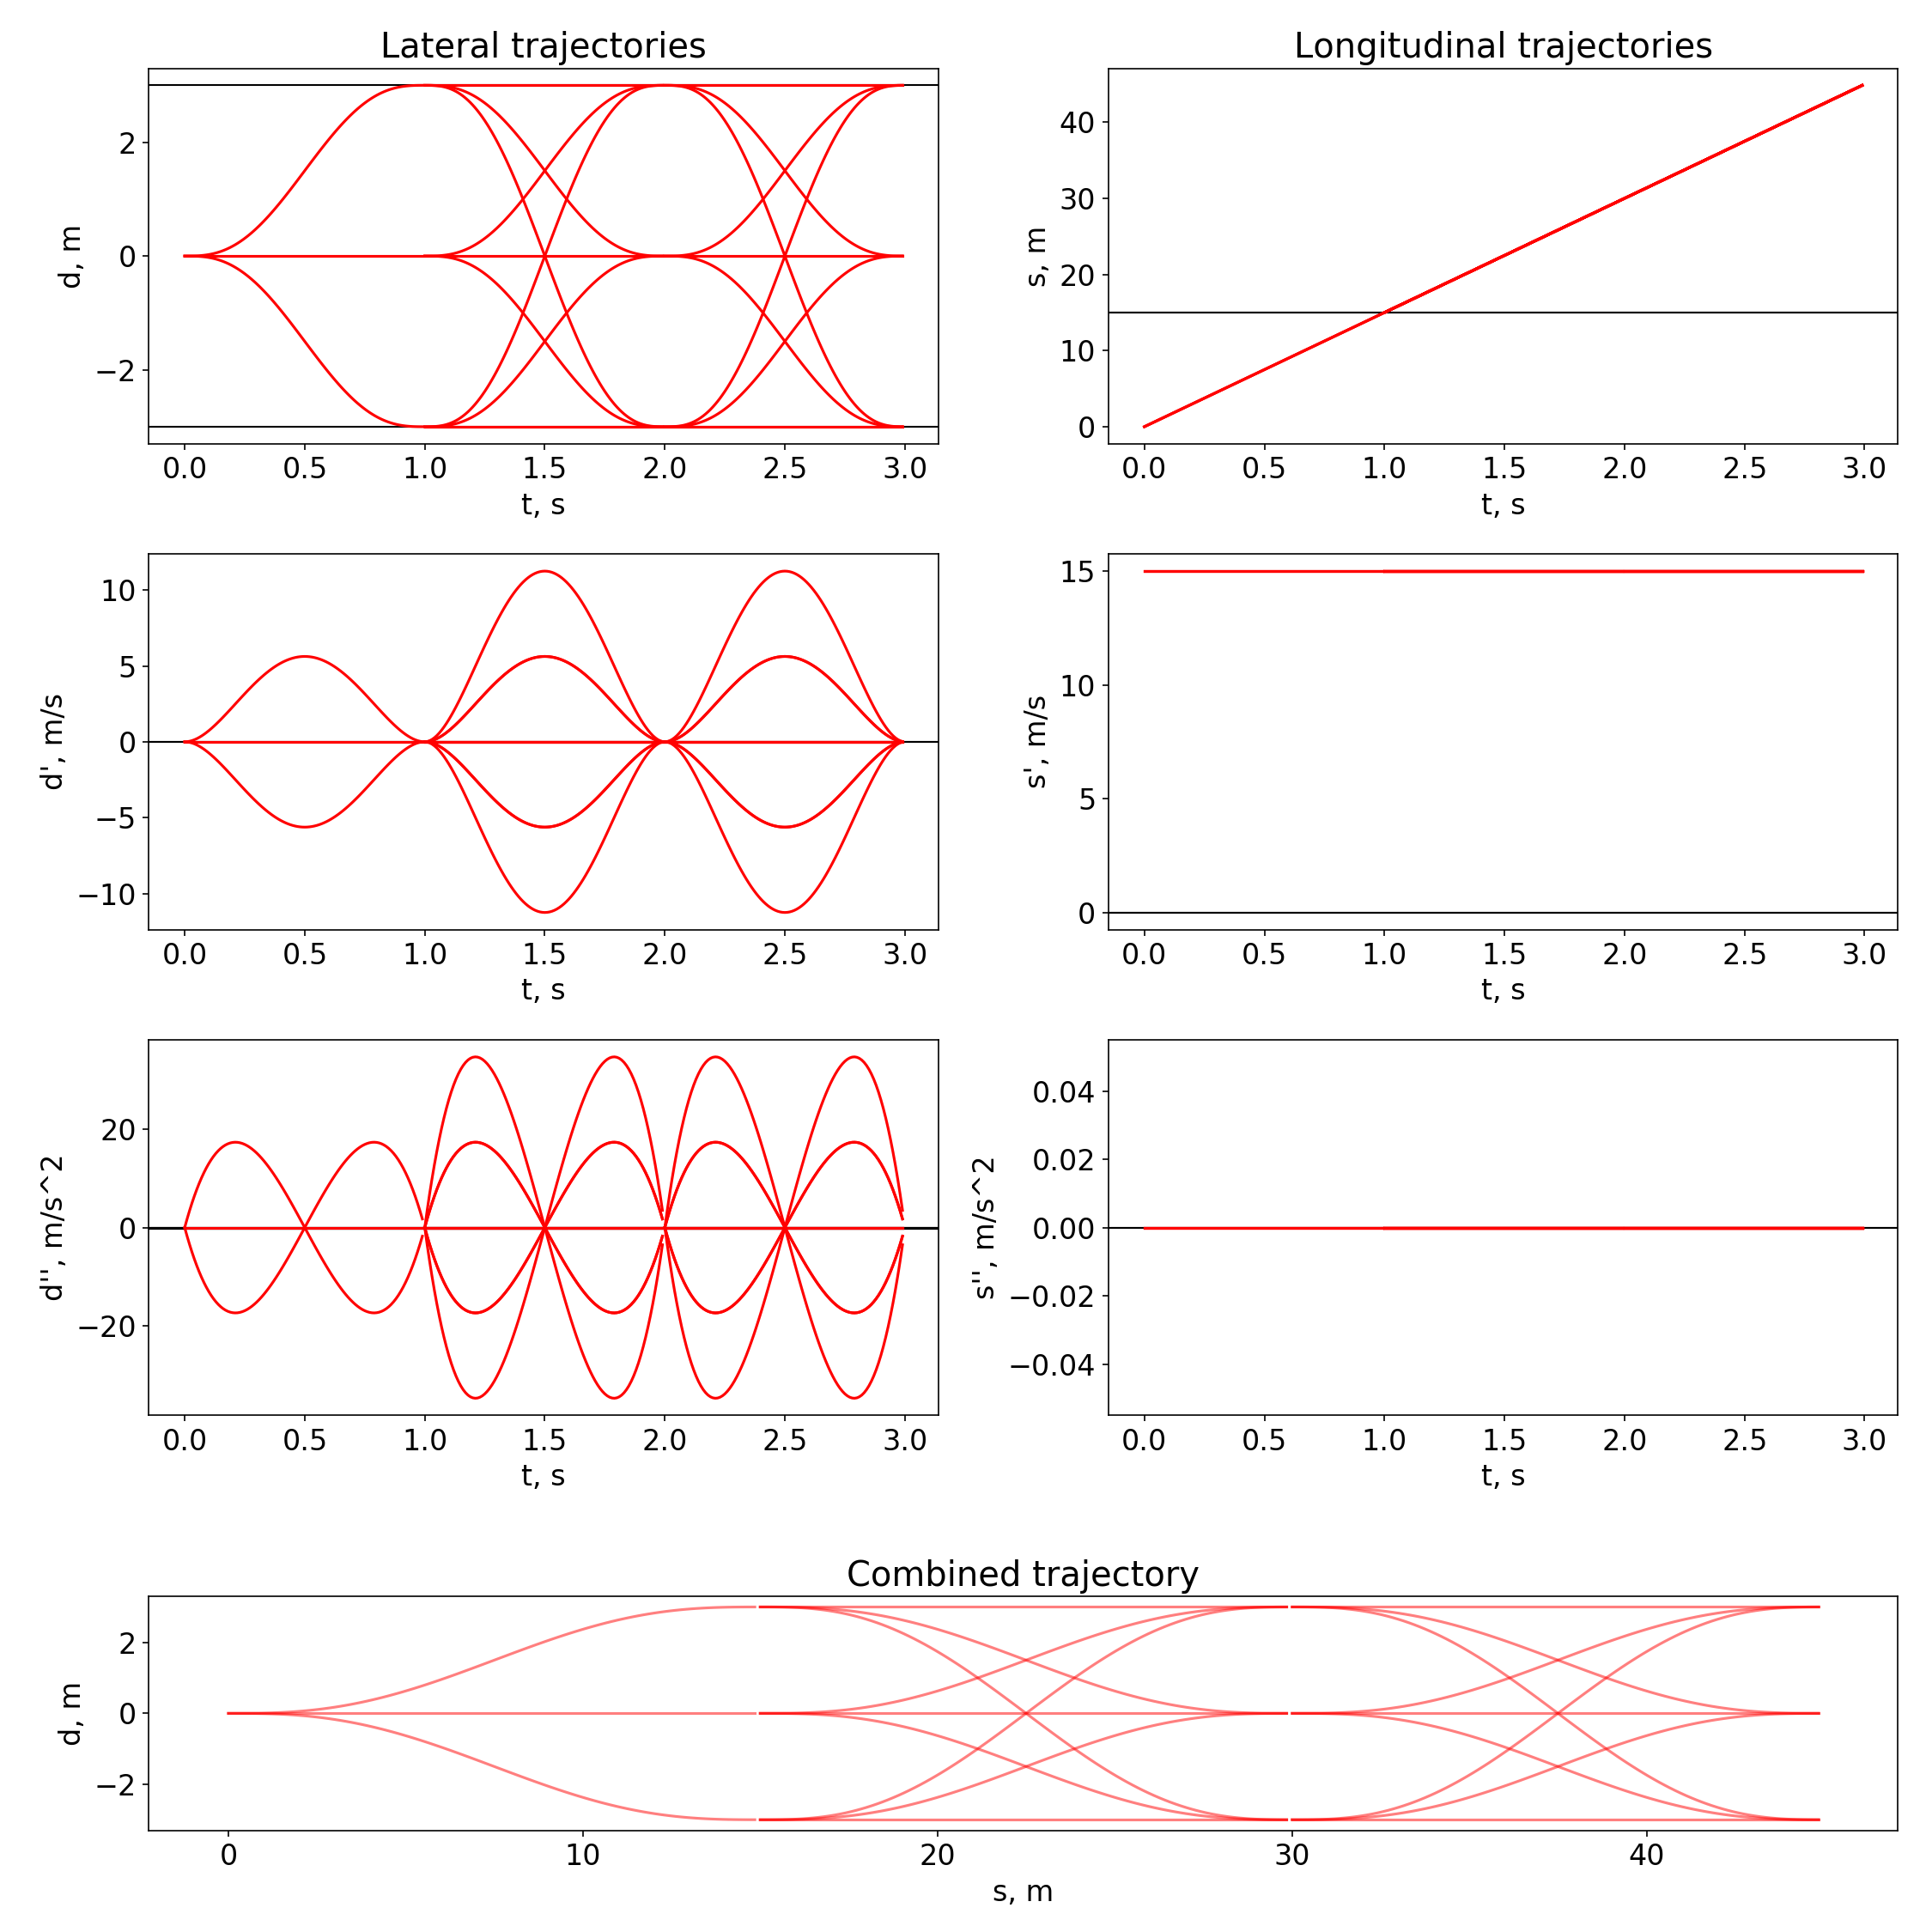
\includegraphics[width=\linewidth]{images/2_project/quintic_2/multistep_trajectories}
            \caption{Пример формирования набора траекторий}
      \label{img:multistep_trajectories}
\end{figure}

% TODO: собственно, надо сделать опять планирование с препятствием

%\section{Проектирование подсистемы следования траектории}
